\chapter{A Quantitative Theory of Uniform Distribution}\label{chap1}

\section[The Uniform Distribution of a sequence...]{The Uniform
  Distribution of a sequence in an interval or in a
  cube}\label{chap1:sec1}\pageoriginale   

Denote by $U$ the unit interval $0 \leq x \leq 1$, and by $I$ any sub-interval of $U$. (We shall allow open, closed, half open intervals, as well as single points and the empty set $\phi$). Denote the length of $I$ by $|I|$. Let $x_{1}, x_{2}, \ldots$ be a sequence of numbers in $U$. For every interval $I$, put
$$
z(n, I) = \sum_{\substack{1\leq i \leq n\\ x_{i} \in I}}\quad 1.
$$

The sequence $x_{1}, x_{2}, \ldots$ is called {\em uniformly distributed}, if for every I we have the asymptotic relation
$$
z(n, I) \thickapprox n |I|,
$$
that is, if $z(n, I)/(n|I|)$ tends to $1$ as $n$ goes to infinity. Set
\begin{align*}
  D(n, I) &= z(n, I) - n|I|,\\
  \triangle(n) &= \sup\limits_{I} |D(n, I)|,
\end{align*}
where the supermum is taken over all the sub-intervals of $U$. The function $\triangle(n)$ is called the {\em discrepancy} function.

Let $\mathfrak{C}$ be a finite collection of sub-intervals of $U$ with $\phi \epsilon \mathfrak{C}, U \epsilon \mathfrak{C}$.

For an arbitrary $I$, write
$$
\delta_{\mathfrak{C}} (I) = \min_{\substack{I_{1}, I_{2} \epsilon \mathfrak{C}\\I_{1} \subseteq I \subseteq I_{2}}} (|I_{2}| - |I_{1}|)
$$

Further set
$$
\delta_{\mathfrak{C}} = \sup\limits_{I} \delta_{\mathfrak{C}} (I),
$$\pageoriginale
where the supermum is taken over all the sub-intervals of $U$, and put
$$
\Delta_{\mathfrak{C}}(n) = \sup\limits_{I \epsilon \mathfrak{C}} |D(n, I)|.
$$

We claim that
\begin{equation*}
\delta(n)\leq \Delta_{\mathfrak{C}} (n) + n\delta_{\mathfrak{C}}\tag{1.1}\label{chap1:sec1:eq1.1}
\end{equation*}

The proof is as follows. Let I be arbitrary. Since $\mathfrak{C}$ is a finite collection, there exist intervals $I_{1}, I_{2} \epsilon \mathfrak{C}$ with
$$
I_{1} \subseteq I \subseteq I_{2}\quad\text{and}\quad|I_{2}| - |I_{1}| \leq \delta_{\mathfrak{C}}.
$$

Now
\begin{align*}
D(n, I) & = z(n, I) - n|I|\\
        & \leq z(n, I_{2}) - n|I_{2}| + n(|I_{2}| - |I|)\\
        & \leq D(n, I_{2}) + n\delta_{\mathfrak{C}}\\
        & \leq \triangle_{\mathfrak{C}} (n) + n\delta_{\mathfrak{C}}.
\end{align*}

A lower bound for $D(n, I)$ may be proved similarly, so that 
$|D(n, I)| \leq \triangle_{\mathfrak{C}} (n) + n\delta_{\mathfrak{C}}.$

Since this is true for every $I$, we get (\ref{chap1:sec1:eq1.1}).

\begin{lemma}\label{chap1:sec1:lem1A}
  A sequence is uniformly distributed if and only if 
  \footnotetext[1]{The notation $g(n) =o(f(n))$ means that $g(n)/f(n) \rightarrow 0$ as $n\to\infty$.}
  $$
  \triangle(n) = o(n) \footnotemark[1].
  $$
\end{lemma}

\begin{proof}
 $\triangle(n) = o(n)$ implies that $D(n, I) = o(n)$ for any $I$, which is equivalent to $z(n, I) \thickapprox n|I|$ for any $I$. Hence the sequence is uniformly distributed.
\end{proof}

To go in the opposite direction, it will be convenient to introduce the symbol $\dot{<}$. The notation $x \dot{<} \beta$ we shall mean $x <\beta$ if $\beta \neq 1$, and $x \leq \beta$ if

$\beta = 1$.\pageoriginale For a positive integer, $h$, denote by $\mathfrak{C}_{h}$ the collection of sub-intervals of $U$ of the type $\dfrac{u}{2^{h}} \leq x \dot{<} \dfrac{v}{2^{h}}$ with integers $u, v$. Since $\mathfrak{C}_{h}$ is a finite collection of intervals, the uniform distribution implies that $\triangle_{\mathfrak{C}_{h}} (n) = o(n)$. Further observe that $\delta_{\mathfrak{C}_{h}} \leq 2.2^{-h}$. Thus for any given $\epsilon > 0$ we can choose $h$ with $\delta_{\mathfrak{C}_{h}} < \dfrac{\epsilon}{2}$. Using (\ref{chap1:sec1}), we obtain
$$
\triangle(n) \leq \triangle_{\mathfrak{C}_{h}} (n) + \dfrac{\epsilon}{2} n.
$$

In view of $\triangle_{\mathfrak{C}_{h}} (n) = o(n)$, we get $\triangle(n) \leq \epsilon n$ for large $n$. This completes the proof of Lemma 1\ref{chap1:sec1:lem1A}.

We are interested in sequences which are very well uniformly distributed, i.e. which have $\triangle(n) \ll f(n)$\footnote{The notation $g(n) \ll f(n)$ (which is due to Vinogradov) means that $|g(n)/f(n)|$ is bounded as a function of $n$.} where $f(n)/(n)$ tends to zero very rapidly. The following is an example of such a sequence. (See also Theorem 1\ref{chap1:sec1:thm1D}.)

Every real number $\mathfrak{J}$ may uniquely be written as a sum
$$
\mathfrak{J} = [\mathfrak{J}] + \{\mathfrak{J}\},
$$   
where $[\mathfrak{J}]$, the ``integer part of $\mathfrak{J}$'', is an integer, and where$\{\mathfrak{J}\}$, the ``fractional part of $\mathfrak{J}$'', satisfies $0 \leq \{\mathfrak{J}\} < 1$.

\begin{theorem}[$^{*}$]\label{chap1:sec1:thm1B}
  \footnote{Theorems with an attached star are not proved in these lectures.}
  \cite{12} Suppose $\alpha$ is a real number which has bounded partial denominators in its continued fraction expansion. Then the sequence $\{\alpha\}, \{2\alpha\}, \{3\alpha\}, \ldots$ has
  $$
  \triangle (n) \ll \log n.
  $$
\end{theorem}
The following result shows that it is not possible to improve

Theorem 1\ref{chap1:sec1:thm1B}${^*}$ (except for giving an explicit value for the constant implies by $\ll$). Recall that the notation

$$
f(n) = \Omega(g(n))
$$\pageoriginale
means that $f(n)/g(n)$ does {\em not} tend to $0$ as $n \to \infty$.

\begin{theorem}[$^{*}$]\label{chap1:sec1:thm1C}
 \cite{8}-\cite{16} For an arbitrary real number $\alpha$, the sequence
$$
\{\alpha\}, \{2\alpha\}, \ldots
$$
has
$$
\triangle(n) = \Omega (\log n).
$$
\end{theorem} 

We now shall study the discrepancy function of the sequence of Vander Corput:
$$
\dfrac{1}{2}, \dfrac{1}{4}, \dfrac{3}{4}, \dfrac{1}{8}, \dfrac{5}{8}, \dfrac{3}{8}, \dfrac{7}{8}, \dfrac{1}{16}, \ldots .
$$

The method of constructing the above sequence is illustrated by the scheme
\begin{align*}
& \frac{1}{2},\\
& \frac{1}{4}, \frac{1}{4} + \frac{1}{2},\\
& \frac{1}{8}, \frac{1}{8} + \frac{1}{2}, \frac{1}{8} + \frac{1}{4}, \frac{1}{8} + \frac{1}{4} + \frac{1}{2}.\\
&\ldots\ldots\ldots\ldots\ldots\ldots\ldots\ldots\ldots.
\end{align*}

\begin{theorem}\label{chap1:sec1:thm1D}
\cite{29} The above sequence has
$$
 \triangle(n) \ll \log n. 
$$
\end{theorem}

\begin{proof}
  Call $I \subseteq U$ an {\em elementary interval} if it is of the type $\dfrac{w}{2^{k}} \leq x \dot{<} \dfrac{w + 1}{2^{k}}$, where $w$ is an integer. For a positive integer $h$, denote by $\mathfrak{C}$ the collection of sub-interval of $U$ of the type $\dfrac{u}{2^{h}} \leq x \dot{<} \dfrac{v}{2^{h}}$, with integers $u, v$. Note that $\delta_{\mathfrak{C}_{h}} \leq 2^{1-h}$.
\end{proof}

We shall show in a moment that
\begin{equation*}
 |D(n, I)|\leq 1|\tag{1.2}\label{chap1:sec1:eq1.2}
\end{equation*}
{\em for every elementary interval} $I$.\pageoriginale

It is readily seen by induction on $h$ that an interval of $\mathfrak{C}_{h}$ is the union of not more than $2h$ disjoint elementary intervals. So (\ref{chap1:sec1:eq1.2}) implies that
$$
\triangle_{\mathfrak{C}_{h}}(n) \leq 2h ,
$$
since the function $D(n, I)$ is additive (i.e., $D(n, I) = D(n, I)+ D(n, I_{2})$, if $I = I_{1} \cup I_{2}$ and $I_{1} \cap I_{2} = \phi$). Using (\ref{chap1:sec1:eq1.1}). we get
$$
\triangle(n) \leq 2h + n 2^{1-h}.
$$

Setting $h = [\log_{2} n]$\footnote{$\log_{2} x$ is the logarithm of $x$ with base  $2$.}
$+ 1$, we obtain
$$
 \triangle(n) \leq 2(\log_{2} n+1) + 2 \leq \frac{2}{\log 2} \log n + 4 \ll \log n.
$$

{\em It remains to prove} (\ref{chap1:sec1:eq1.2}). Let $I$ be the arbitrary elementary interval $\frac{w}{2^{k}} \leq x \dot{<} \frac{w+1}{2^{k}}$. Write the integer $n$ in the dyadic scale,
$$
n = a_{t} \ldots a_{0}.
$$

Notice that Vander Corput's sequence $x_{1} = \frac{1}{2}, x_{2} = \frac{1}{4} \ldots$ has 
$$
x_{n} = 0. \quad a_{0} \ldots a_{t}\qquad\text{(in the dyadic scale).}
$$

It follows that $x_{n} \epsilon I$ precisely if $w$ above has the dyadic expansion $w = a_{0}a_{1} \ldots a_{k - 1}$. Thus for fixed $w$, we have $x_{n} \epsilon I$ precisely if n lies in a certain fixed residue class $\mod 2^{k}$. Hence
$$
D(n, I) = |z(n, I) - \frac{n}{2^{k}}| \leq 1 .
$$

This completes the proof of Theorem 1\ref{chap1:sec1:thm1D}.

Now we generalise to $k$ dimensions. Points in k - dimensional space
will\pageoriginale be written as $\uub{x}= (x_{1}, \ldots, x_{k})$. Denote by $U^{k}$ the unit cube consisting of $\uub{x}= (x_{1}, \ldots, x_{k})$ 
with $x_{i} \epsilon U (1 \leq i \leq k)$.

A set $B \subseteq U^{k}$will be called a {\em box} if it is a Cartesian product $I_{1} \times \ldots \times I_{k}$ of intervals $I_{1}, \ldots, I_{k}$. If, for example, $I_{j} = [a_{j}, b_{j}], 1\leq j \leq k$, then $B$ consists of $\uub{x}= (x_{1}, \ldots, x_{k})$ 
with $a_{j} \leq x_{j} \leq b_{j} (j = 1, \ldots, k)$.

Let $\uub{x}_{1}, \uub{x}_{2}, \ldots$ be a sequence of points in $U^{k}$. Given a box $B$, put 
$$
z(n, B) = \sum_{\substack{1 \leq i \leq n\\\uub{x_{i}} \epsilon B}}1.
$$

The sequence $\uub{x}_{1}, \uub{x}_{2}, \ldots$ is called {\em uniformly distributed}, if for every box $B$ we have the asymptotic relation
$$
z(n, B) \thickapprox n|B|,
$$
where $|B|$ denote the volume of $B$. Set
\begin{align*}
D(n, B) & = z(n, B) - n|B|,\\
\triangle(n) & = \sup_{\substack{B}} |D(n, B)|,
\end{align*}
where the supremum is taken over all the boxes $B$ in $U^{k}$. Here $\triangle(n)$ is called the {\em discrepancy} function.

Let $\mathfrak{C}$ be a finite collection of boxes with $\phi \epsilon \mathfrak{C}, U^{k} \epsilon \mathfrak{C}$. For an arbitrary box B, define
\begin{align*}
\delta_{\mathfrak{C}}(B) & = \sup_{\substack{B_{1}, B_{2} \epsilon \mathfrak{C}\\B_{1} \subseteq B \subseteq B_{2}}} (|B_{2}| - |B_{1}|),\\
 \delta_{\mathfrak{C}} & = \sup_{\substack{B}} \delta_{\mathfrak{C}}(B),
\end{align*}
where\pageoriginale the supremum is taken over all the boxes $B$ in $U^{k}$, and put
$$
\triangle_{\mathfrak{C}}(n) = \sup_{\substack{B \epsilon \mathfrak{C}}} |D(n, B)|.
$$

We remark that the the inequality (\ref{chap1:sec1:eq1.1}) can be established in this general set-up, and Lemma 1\ref{chap1:sec1:lem1A} can also be generalised.

Given a point $\uub{x} = (x_{1}, \ldots, x_{k})$, write
$$
\uub{x} = (\{x_{1}\}, \ldots \{x_{k}\}).
$$

Let $\uub{\alpha}$ be arbitrary in $k$-dimensional space, and consider the sequence $\{\uub{\alpha}\}, \{2\uub{\alpha}\}, \ldots$. One would like to have points $\uub{\alpha}$ fro which this sequence has $\triangle(n) \ll (\log n)^{k}$. If $k > 1$, it is not known whether such an $\uub{\alpha}$ exists, and hence there is no satisfactory analogue of Theorem 1\ref{chap1:sec1:thm1B}. It is not even known if an $\uub{\alpha}$ exists for $k > 1$ such that $\triangle(n) \ll (\log n)^{k+1}$. However, it was proved \cite{20} that for ``almost every $\uub{\alpha}$'' (in the sense of Lebesgue measure) $\triangle(n) \ll (\log n)^{k+1+\epsilon}$ for every $\epsilon > 0$.

Like for Theorem 1\ref{chap1:sec1:thm1B}${^*}$, no satisfactory analogue of Theorem 1\ref{chap1:sec1:thm1C}$^{*}$ is known. For an analogue of Theorem $1D$, we now turn to the sequence of Hammersley \cite{7}.

Let $p_{1}, \ldots, p_{k}$ be integers greater than $1$ and relatively prime in pairs (i.e., $(p_{i}, p_{j}) = 1$ whenever $i \neq j$). (The simplest choice is to take $p_{1}, \ldots , p_{k}$ to be the first $k$ primes). For a positive integer $n$, write 
$$
\begin{matrix}
n = a_{w_{1}}^{(p_{1})} \ldots a_{0}^{(p_{1})}\qquad\text{(in the scale of} p_{1}),\\
\hdotsfor{1}\\
\hdotsfor{1}\\
n = a_{w_{k}}^{(p_{k})} \ldots a_{0}^{p_{k}}\qquad\text{(in the scale of} p_{k}).
\end{matrix}
$$

Put
$$
\begin{matrix}
x_{n1} = 0.a_{0}^{(p_{1})} \ldots a_{w_{1}}^{(p_{1})}\qquad\text{(in the scale of} p_{1})\\
\hdotsfor{1}\\
\hdotsfor{1}\\
x_{nk} = 0.a_{0}^{(p_{k})} \ldots a_{w_{k}}^{(p_{k})}\qquad\text{(in the scale of} p_{k}).
\end{matrix}
$$\pageoriginale

Set 
$$
\uub{x}_{n} = (x_{n1}, \ldots, x_{nk})\qquad(n = 1, 2, \ldots)
$$

The sequence $\uub{x}_{1}, \uub{x}_{2}$ so constructed is called {\em
  Hammersley's seque\-nce}. (For $k = 1$, $p_{1} = 2$ it gives Van der
Corput's sequence). 

\begin{theorem}\label{chap1:sec1:thm1E}
\cite{6} Hammersley's sequence has
$$
\triangle(n) \ll (\log n)^{k}.
$$
\end{theorem}

\begin{proof}
 Let $\mathfrak{C}_{h}^{j} (1 \leq j \leq k)$ be the collection of intervals in $U$ of the type $\frac{u}{p_{j}^{h}} \leq x \dot{<} \frac{v}{p_{j}^{h}}$, with integers $u, v$. Let $\mathfrak{C}_{h} = \mathfrak{C}_{h}^{1} \times  \ldots \times  \mathfrak{C}_{h}^{k}$, i.e. let $\mathfrak{C}_{h}$ be the collection of all the boxes $B = I_{1} \times \ldots \times I_{k}$ with $I_{j} \epsilon \mathfrak{C}_{h}^{j} (j = 1, \ldots , k)$.
\end{proof}

We claim that
\begin{equation*}
 \delta_{\mathfrak{C}_{h}} \leq \delta_{1_{\mathfrak{C}_{h}}} + \ldots + \delta_{k_{\mathfrak{C}_{h}}}.\tag{1.3}\label{chap1:sec1:eq1.3}
\end{equation*}

Let $B = I_{1} \times \ldots \times I_{k}$ be an arbitrary box. Choose intervals
$$
I_{1}^{1}, \ldots, I_{1}^{k} ; I_{2}^{1}, \ldots, I_{2}^{k}
$$
such that
$$
I_{1}^{i} \subseteq I_{j} \subseteq I_{2}^{j}, I_{1}^{j}, I_{2}^{j} \epsilon \mathfrak{C}_{h}^{j} (j = 1, \ldots , k).
$$
and
$$
|I_{2}^{j}|-|I_{1}^{j}| \leq \delta_{\mathfrak{C}_{h}^{j}} (j = 1, \ldots, k).
$$

Set\pageoriginale $B_{1} = I_{1}^{1} \times \ldots \times I_{1}^{k}$ and $B_{2} = I_{2}^{1} \times \ldots \times I_{2}^{k}$. Then $B_{1} \subseteq B \subseteq B_{2}$ and $B_{1}, B_{2} \epsilon \mathfrak{C}_{h}$. 

Further observe that
$$
\delta_{\mathfrak{C}_{h}} (B) \leq |B_{2}| - |B_{1}| \leq \delta_{\mathfrak{C}_{h}^{1}} + \ldots + \delta_{\mathfrak{C}_{h}^{k}}.
$$ 

Since this is true for any box $B \epsilon \mathfrak{C}_{h}$, we obtain (\ref{chap1:sec1:eq1.3}).

Notice that $\delta_{\mathfrak{C}_{h}^{j}} \leq 2p_{j}^{-h} (1 \leq j \leq k)$, and so $(1.3)$ gives
\begin{equation*}
 \delta_{\mathfrak{C}_{h}} \leq 2(p_{1}^{-h} + \ldots + p_{k}^{-h}) \leq 2^{1-h} k.\tag{1.4}\label{chap1:sec1:eq1.4}
\end{equation*}

An interval of the type $\frac{w}{p_{j}^{t}} \leq x \dot{<} \frac{w+1}{p_{j}^{t}}$, where $w$ is an integer, is called an {\em elementary} $p_{j}$ -{\em type interval}. A box $B = I_{1} \times \ldots \times I_{k}$ is called an elementary box if each $I_{j}$ is an {\em elementary} $p_{j}$ -type interval.

Let $B = I_{1} \times \ldots \times I_{k}$ be an elementary box with $I_{j}$ given by 
$$
\frac{w_{j}}{p_{j}^{t_{j}}} \leq x < \frac{w_j +1}{p_{j}^{t_{j}}} (1 \leq j \leq k).
$$

Thus $\uub{x}_{n} \epsilon B$ if and only if
$$
\frac{w_j+1}{p_{j}^{t_{j}}} \leq x_{nj} < \frac{j^{w+1}}{p_{j}^{t_{j}}} (1 \leq j \leq k).
$$

Since $x_{nj} < 1$ for the Hammersley sequence, we may replace $\dot{<}$ by $<$ here. For fixed $j$, the inequalities above determine $t_{j}$ digits in the expansion of $x_{nj}$ in the scale of $p_{j}$, hence determines $t_{j}$ digits in the expansion of $n$ in the scale of $p_{j}$. Thus for fixed $j$, the inequalities hold if and if $n$ lies in a fixed residue class modulo $p_{j}^{t_{j}}$. Hence by the Chinese Remainder Theorem, $\uub{x}_{n} \in B$ precisely if $n$ lies in a fixed residue class modulo $p_{1}^{t_{1}} \ldots p_{k}^{t_{k}}$.

Hence\pageoriginale
\begin{equation*}
  D(n, B) = |z(n, B) - \frac{n}{p_{1}^{t_{1}} \ldots p_{k}^{t_{k}}}| \leq 1.\tag{1.5}\label{chap1:sec1:eq1.5}
\end{equation*}

As is easily seen by induction on $h$, every interval $I$ of $\mathfrak{C}_{h}^{i}$ is a dis-joint union of not more than $2(p_{i}-1)h < 2p_{i}h$ elementary $p_{i}$-type intervals.

Hence every box $B$ of $\mathfrak{C}_{h}$ is the union of not more than $(2p_{1}h) \ldots$ $(2p_{k}h) = (2h)^{k} p_{1} \ldots p_{k}$ elementary boxes. We therefore see form (\ref{chap1:sec1:eq1.1}), (\ref{chap1:sec1:eq1.4}) and (\ref{chap1:sec1:eq1.5}) that
$$
\triangle(n) \leq (2h)^{k} p_{1} \ldots p_{k} + n2^{1-h}k.
$$

Setting $h = [\log_{2} n] + 1$, we get
$$
\triangle(n) \leq (2 \log_{2} n + 2)^{k} p_{1} \ldots p_{k} + 2k \ll (\log n)^{k}.
$$

\section{Roth's Theorem}\label{chap1:sec2}

Assume $k = 1$. One can ask if there exists a sequence with $\triangle(n) \ll 1$. Van der Corput \cite{29} conjectured that $\triangle(n) \ll 1$ is impossible.
Aardenne-Ehrenfest \cite{1} proved the conjecture. Later \cite{2} she further showed that $\triangle(n) = \Omega (\log \log n/ \log \log \log n)$. Then K. F. Roth \cite{19} improved it to $\Omega (\sqrt{\log n})$ and W. M. Schmidt \cite{25} to $\Omega(\log n)$.

When $k$ is arbitrary, $\triangle(n) = \Omega((\log n)^{k/2})$, which is contained in the following theorem of K. F. Roth \cite{19}.

\begin{theorem}\label{chap1:sec2:thm2A}
Let $\uub{x}_{1}, \uub{x}_{2}, \ldots$ be a sequence in $U_{k}$. If $N > c_{k}$, then there exists an $n$, $1 \leq n \leq N$, such that
\begin{equation*}
  \triangle(n) > c'_{k} (\log N)^{k/2} .\tag{2.1}\label{chap1:sec2:eq2.1}
\end{equation*}
Here $c_{k} > 0, c'_{k} > 0$
are constants depending only on $k$.
\end{theorem}

\begin{remark*}
It follows from Theorem 2\ref{chap1:sec2:thm2A} that there exist infinitely many $n$\pageoriginale satisfying $\triangle(n) > c'_{k} (\log n)^{k/2}$. If $n, 1 \leq n \leq N$, satisfies (\ref{chap1:sec2:eq2.1}), then $n \geq \triangle (n) \geq c'_{k} (\log N)^{k/2}$, and so $n \to \infty$ as $N \to \infty$. Hence $\triangle (n) = \Omega ((\log n)^{k/2})$.
\end{remark*}

Let $\uub{p}_{1}, \ldots, \uub{p}_{N}$ be N points in $U^{k}$. If A is a measurable subset of $U^{k}$ with measure $\mu (A)$, put $Z(A)$ for the number of $i(1 \leq i \leq N)$ for which $\uub{p}_{i} \epsilon A, D(A) = Z(A) - N(A) - N \mu (A)$.

\begin{theorem}\label{chap1:sec2:thm2B}
 There exists a box B with
$$
|D(B)| > d'_{k} (\log N)^{(k - 1)/2} \qquad\text{if}\quad N > d_{k}.
$$
\end{theorem}

Here $d_{k} > 0$, $d'_{k} > 0$ are constants depending only on $k$.

Roth observed: {\em The case} $k$ of Theorem 2\ref{chap1:sec2:thm2A} is equivalent to the case $(k+1 )$ of Theorem 2\ref{chap1:sec2:thm2B}. We shall prove this equivalence for $k = 1$, as the proof for arbitrary $k$ is similar. We shall first show that

THEOREM 2\ref{chap1:sec2:thm2B} with $k = 2$ implies THEOREM 2\ref{chap1:sec2:thm2A} with $k = 1$.

BY Theorem 2\ref{chap1:sec2:thm2B} with $k = 2$, there exists for large $N$ a box $B$ satisfying
\begin{equation*}
  |D(B)| > d'_{2} \sqrt{\log N}.\tag{2.2}\label{chap1:sec2:eq2.2}
\end{equation*}

Introduce the notations $B(x, y) = [0, x] \times [0, y]$, $B(x-, y) = [0, x) \times [0, y]$, $B(x, y-) = [0, x] \times [0, y)$ and $B(x-, y-)= [0, x) \times [0, y)$ for boxes. Put
\begin{align*}
  Z(x, y) & = Z(B,(x, y))\\
  D(x, y) & = D(B(x, y)) = Z(x, y) - Nxy.
\end{align*}

Similarly define $Z(x-, y), D(x-, y)$, etc. Assume at the moment that the box $B$ of (\ref{chap1:sec2:eq2.2}) is of the type
$$
B:(\zeta, \eta), a < \zeta \leq b, c < \eta \leq d.
$$

Then
$$
Z(B) = Z(b, d) - Z(a, d) - Z(b, c) + Z(a, c).
$$
and therefore\pageoriginale
$$
D(B) =  D(b, d) - D(a, d) - D(b, c) + D(a, c).
$$

Since $|D(B)| > d'_{2} \sqrt{log N}$, there exists a point $(x_{0}, y_{0})$ (with $x_{0} = a$ or $b$, $y_{0} = c$) such that
$$
|D(x_{o}, y_{0})| > \frac{d'_{2}}{4} \sqrt{\log N}.
$$

If B is of some other type, we may come up with, say,
$$
|D(x_{o}-, y_{0})| > \frac{d'_{2}}{4} \sqrt{\log N}.
$$

If $D(x_{0}-, y_{0}) > 0$, then $D(x_{0}, y_{0}) \geq D(x_{0}-, y_{0}) > \frac{d'_{2}}{4}\sqrt{\log N}$. If $D(x_{0}-, y_{0}) < 0$, choose $\hat{x_{0}}$ with $x_{0} - \frac{1}{N} (|D(x_{0}-, y_{0})| - \frac{d'_{2}}{4}\sqrt{\log N}) < \hat{x_{0}} < x_{0}$. Then $|D(\hat{x_{0}}, y_{0})| \geq -D(\hat{x_{0}}, y_{0}) = N\hat{x_{0}}y_{0} - Z(\hat{x_{0}}, y_{0}) \geq Nx_{0}y_{0} - Z(x_{0}-, y_{0}) - Ny_{0}(x_{0} - \hat{x_{0}}) > |D(x_{0}-, y_{0})| - (|D(x_{0}-, y_{0}))| - \frac{d'_{2}}{4}\sqrt{\log N}) = \frac{d'_{2}}{4}\sqrt{\log N}$.

In this way one sees that there is always on $x_{0}, y_{0}$ with $|D(x_{0}, y_{0})| > \sqrt[c]{\log N}$ with $x = d'_{2}/4$.

Let $x_{1}, \ldots, x_{N}$ be in $U^{1} = U$. Apply what we just said to the $N$ points $\uub{p}_{1} = (x_1, \frac{1}{N}), \ldots, \uub{p}_{N} = (x_{N}, \frac{N}{N})$. Let $(x_0, y_{0})$ be such that
$$
|D(x_{0}, y_{0})| > \sqrt[c]{\log N}.
$$

Let $I$ be the interval $0 \leq x \leq x_{0}$. Put $n = [Ny_{0}]$. Then $1 \leq n \leq N$ is large. 

For if we had $n = 0$, then $y_{0} < 1/N$, whence $1 > |Nx_{0}y_{0}| = |D(x_{0}, y_{0})| > \sqrt[c]{\log N}$. which is not possible for large $N$. Observe that 
\begin{align*}
  z(n, I) & = \text{the number of i with} 1 \leq i \leq n, x_{i} \epsilon I, \quad{\text hence}\\
  & = \text{the number of i for which}~ \uub{p}_i = (x_i, \frac{i}{N})\qquad\text{has}\\
  & \quad 0 \leq x_{i} \leq x_{0}, \frac{i}{N} \leq \frac{n}{N}, \quad\text{hence}\\
  & = Z\left(x_{0}, \frac{n}{N}\right)\\
  & = Z(x_{0}, y_{0}),\quad\text{since} \frac{n}{N} \leq y_{0} < \frac{n+1}{N}.
\end{align*}

Further\pageoriginale
\begin{align*}
|D(n, I)| & = |z(n, I) - n|I||\\
 & = |Z(x_{0}, y_{0}) - [Ny_{0}]x_{0}|\\
 & \geq |Z(x_{0}, y_{0}) - Nx_{0}y_{0}| - |Nx_{0}y_{0} - [Ny_{0}]x_{0}|\\
 & \geq |D(x_{0}, y_{0})| - 1 > \frac{c}{2} \sqrt{\log N},\text{ if }
\end{align*}
$N$ is large. Thus $\triangle(n) > \frac{c}{2} \sqrt{\log N}$.

We next are going  to show that
THEOREM 2\ref{chap1:sec2:thm2A} with $k = 1$ implies THEOREM 2\ref{chap1:sec2:thm2B} with $k = 2$.

Let $\uub{p}_{1} = (x_{1}, y_{1}), \ldots ,\uub{p}_{N} = (x_{N}, y_{N})$ be any $N$ points in $U^{2}$. We may assume, without loss of generality, that
$$
y_{1} \leq y_{2} \ldots \leq y_{N}.
$$

We construct new points
$$
\uub{p}_{1}^{*} = (x_{1}, \frac{1}{N}), \ldots, \uub{p}_{N}^{*} = (x_{N}, \frac{N}{N}).
$$

Apply Theorem 2\ref{chap1:sec2:thm2A}, with $k = 1$, to the points $x_{1}, \ldots x_{N}$; there exists an integer $n$, $1 \leq n \leq N$, such that
$$
\triangle(N) > c'_{1} \sqrt{\log N}.
$$
i. e., there exists an interval $I$ with
$$
|z(n, I) - n|I|| > c'_{1} \sqrt{\log N}.
$$

Suppose $I$ is, say, $a < x \leq b$. If we define $z(n, x)$ as the number of $i$ in $1 \leq i \leq n$ with $0 \leq x_{i} \leq x$, then
$$
z(n, I) - n |I| = (z(n, b) - nb) - (z(n, a) - na).
$$ 

So there exists an $x_{0}$ (namely $x_{0} = a$ or $x_{0} = b$) with
$$
|z(n, x_{0}) - nx_{0}| > \frac{c'_{1}}{2} \sqrt{\log N}.
$$

Even\pageoriginale if $I$ is of any other type, we can conclude that there exists an $x_{0}$ with the above property.

Let 
\begin{align*}
M & = \sup_{\substack{(x, y)\epsilon U^{2}}} |Z(x, y) -Nxy|,\\
M^{*} & = \sup_{\substack{(x, y) \epsilon U^{2}}} |Z^{*}(x, y) -Nxy|,
\end{align*}
where $Z^{*} (x, y)$ is the number of $i (1 \leq i \leq N)$ with $\uub{p}_{i}^{*} \epsilon B(x, y)$. Put $y_{0} = \frac{n}{N}$.

Note that $Z^{*} (x_{0}, y_{0}) = z(n, x_{0})$ and
$$
|Z^{*} (x_{0}, y_{0}) - Nx_{0}y_{0}| = |z(n, x_{0}) - nx_{0}| > \frac{c'_{1}}{2} \sqrt{\log N}.
$$

Hence
$$
M^{*} > \frac{c'_{1}}{2} \sqrt{\log N}.
$$

If we can show that $|M - M^{*}| \leq 3M$, then we are through, since then $M \geq \frac{1}{4} M^{*} \geq \frac{c'_{1}}{8} \sqrt{\log N}$. So {\em what remains to be proved is that} $|M - M^{*}| \leq 3M$.

Observe that for every $(x, y) \epsilon U^{2}$,
$$
|Z(x, y) - Z^{*} (x, y)| \leq \max (t, t'),
$$
where $t$ denotes the number of $i$ with $y_{i} \leq y < \frac{i}{N}$ and $t'$ the number of $i$ with $\frac{i}{N} \leq y < y_{i}$. It suffices to prove that $\max (t, t') \leq 3M$, since
$$
\Big||Z(x, y) - Nxy| - |Z^{*}(x, y) - Nxy|\Big| \leq \big|Z(x, y) - Z^{*}(x, y)\big|.
$$

From the definition of $M$, at most $2M$ numbers $y_{i}$ can be equal. (If more than 2M were equal, either $Z(1, 0) > 2M$ whence $|Z(1, 0) - N. 1.0| > 2M$, which is impossible. Or $Z(1, y)$ would have a `jump' greater than $2M$ for some $y > 0$, hence $Z(1, y) - Ny$ would have a `jump' $> 2M$ and $\displaystyle{\sup\limits_{\substack{0 \leq y \leq 1}}}|Z(1, y) - Ny|> M$, which contradicts the definition of $M$). It follows that
$$
|Z(1, y_{i}) - i| \leq 2M - 1\qquad(1 \leq i \leq N).
$$\pageoriginale

By the definition of M, 
$$
|Z(1, y_{i}) - ny_{i}| \leq M \qquad (1 \leq i \leq N).
$$

Combining the above two inequalities, we obtain
\begin{equation*}
  |Ny_{i} - i| \leq 3M - 1 \qquad (1 \leq i \leq N)\tag{2.3}\label{chap1:sec2:eq2.3}
\end{equation*}

By the definition of $t$,
$$
y_{j+1} \leq \ldots y_{j+t} \leq y < \frac{j+1}{N} \ldots < \frac{j+t}{N}.
$$

Observe that
$$
j+t = j+1+ (t-1) > Ny + (t-1), y_{j+t} N \leq Ny.
$$

Combining these inequalities, we obtain
$$
|(j+t) - Ny_{j+t}| \geq (t-1).
$$

This last inequality together with (\ref{chap1:sec2:eq2.3}) yields $t \leq 3M$. Similarly $t' \leq 3M$. Hence $\max (t, t') \leq 3M$. This completes the proof.

More generally, one sees that Theorem 2\ref{chap1:sec2:thm2A} for a particular $k$ is equivalent to Theorem 2B with $k+1$. Since Theorem 2\ref{chap1:sec2:thm2B} is trivial for $k=1$, the Theorem 2\ref{chap1:sec2:thm2A} and 2\ref{chap1:sec2:thm2B} are equivalent. 

Let $uub{y}_{1}, uub{y}_{2}, \ldots$ be Hammersley's sequence in $(k-1)$ -dimen\-sional space.

This sequence has $\triangle(n) \ll (\log n)^{k-1}$. The points $\uub{x}_{1}= (\uub{y}, \frac{1}{N}), \uub{x}_{2} = (\uub{y}_{2}, \frac{2}{N}), \ldots, \uub{x}_{N} = (\uub{y}_{N}, 1)$ lie in $U^{k}$. An argument given above shows that
$$
|D(B)| \leq \overline{c}_{k} (\log N)^{k-1}
$$
for every box $B$ with sides parallel to the axes.

\begin{theorem}[ (Roth)]\label{chap1:sec2:thm2C} 
Let $\uub{p}_{1}, \ldots, \uub{p}_{N}$ be $N$ points in $U^{k}$. Put
$Z(x_{1}$, $\ldots,\break x_{k})$ for the number of $i, 1 \leq i \leq N$,
for which $\uub{p}_{i}$ lies in the box $B(x_{1}, \ldots,\break
x_{k})$\pageoriginale consisting of points $\uub{p} = (p_{1}, \ldots,
p_{k})$ with $0 \leq p_{j} \leq x_{j}(j=1, \ldots, k)$. 
\end{theorem}

If $N > e_{k}$, then 
$$
\int_{U^{k}} \ldots \int (Z(x_{1}, \ldots, x_{k}) - Nx_{1} \ldots x_{k})^{2} dx_{1} \ldots dx_{k} > e'_{k} (\log N)^{k-1}.
$$

Here $e_{k} > 0, e'_{k} > 0$ are constants depending only on $k$.

In particular, there exists a k-tuple $(x_{1}, \ldots, x_{k})$ with
$$
|Z(x_{1}, \ldots, x_{k}) - Nx_{1} \ldots x_{k}| > \hswastic{e'_{k}}(\log N)^{(k-1)/2}.  
$$

Hence Theorem 2\ref{chap1:sec2:thm2C} implies Theorem 2\ref{chap1:sec2:thm2B}.

[Added in June 1976: Recently W. M. Schmidt in a manuscript ``Irregularities of Distribution X'' extended Theorem 2\ref{chap1:sec2:thm2C} by showing that for $r > 1$, 
$$
\int_{U^{k}} \ldots \int \big|Z(x_{1}, \ldots, x_{k}) - Nx_{1} \ldots x-{k}\big|^{r} dx_{1} \ldots dx_{k} > e'_{kr} (\log N)^{(k-1)r/2}.
$$

Moreover, for $k>1$,
\begin{multline*}
\int_{U^{k}} \ldots \int \big|Z(x_{1}, \ldots, x_{k}) - Nx_{1} \ldots x_{k}\big| dx_{1} \ldots dx_{k}\\ 
> e''_{k} \log \log N/\log \log \log N.]
\end{multline*}

\section{Proof of Roth's Theorem}\label{chap1:sec3}

We shall prove Theorem 2\ref{chap1:sec2:thm2C}. For convenience we shall restrict ourselves to the case $k = 2$. We have to show that
$$
\int_{0}^{1} \int_{0}^{1} (Z(x, y) - Nxy)^{2} dx dy > e'_{2} \log N
$$
if $N$ is large. For $x \epsilon U$, write
$$
x = \sum_{j=0}^{\infty} \beta(x) 2^{-j}\quad\text{ (dyadic expansion), }
$$ 
where $\beta_{j}(x)$ is $0$ or $1$. Assume that $\beta_{j}(x)$ never equals $1$ for all $j \geq j_{0}$, except for $x = 1$. Then the dyadic expansion for $x$ is unique. Put
$$
\psi_{r}(x) = (-1)^{\beta_{r}(x)} \quad(r = 1, 2, \ldots).
$$

(The $\psi_{r}(x)$ are called `Rademacher - functions'.)

Let\pageoriginale $\uub{p}_{1} = (x_{1}, y_{1}), \ldots, \uub{p}_{N} = (x_{N}, y_{N})$ be any $N$ points in $U^{2}$. Let $n > 1$ be an integer. Further assume that $r$ is an integer with $0 < r < n$.

For $(x, y) \epsilon U^{2}$, set
$$ F_{r} (x, y) =
\begin{cases}
0, & \text{if there is a }\uub{p}_{i} = (x_{i}, y_{i}) \text{with}\\ 
   & \psi_{1}(x_{i}) = \psi_{1}(x), \ldots, \psi_{r-1}(x_{i}) = \psi_{r-1}(x),\\
   & \psi_{1}(y_{i}) = \psi_{1}(y), \ldots \psi_{n-r-1}(y_{i}) = \psi_{n-r-1}(y).\\
& \psi_{r}(x) \psi_{n-r}(y),\quad\text{ otherwise }.
\end{cases}
$$

We explain the function $F_{r} (x, y)$ with the help of the following diagram.
\begin{figure}[H]
\centering{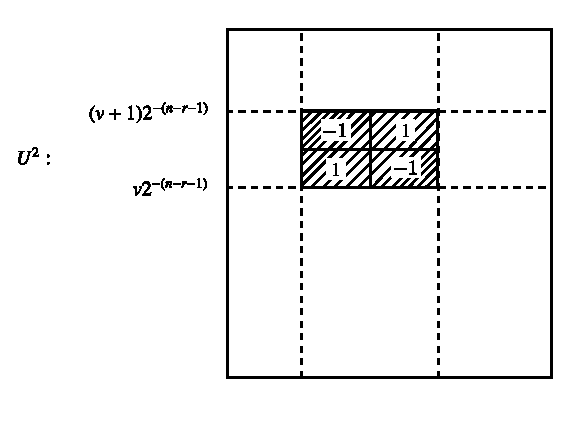
\includegraphics{fig1.eps}}
\end{figure}

Here $u, v$ are integers. $F_{r} (x, y) = 0$, if there is a point $\uub{p}_{i}$ in the shaded ``big'' rectangle $A$. If there is no point $\uub{p}_{i}$ in the $A$, then $F_{r} (x, y) = \pm 1$ in the pattern shown, i. e. , it is $+1$ and $-1$ in two of the four ``small'' rectangles in $A$.\footnote{These rectangles include their left and their lower edge, but not their right and upper edge, except when they adjoin the right or upper edge of $U^{2}$}

Let $y$ be fixed and let $I$ be an interval whose end points are integral multiples of $2^{-(r-1)}$. Then
$$
\int_{I} F_{r} (x, y) dx = 0.
$$\pageoriginale 

This is true because in any interval
$$
u2^{-(r-1)} < x < (u+1)2^{-(r-1)},
$$
either $F_{r}(x, y) = 0$, or $F_{r}(x, y) = \pm 1$ in sub - intervals of equal length.

Similarly fix $x$ and take an interval $I$ whose end points are integral multiples of $2^{-(n-r-1)}$. Then
$$
\int_{I} F_{r} (x, y)dy = 0.
$$

Define $F(x, y)$ for $(x, y) \epsilon U$ by
$$
F(x, y) = \sum_{0 < r < n} F_{r} (x, y).
$$

The proof of Theorem 2\ref{chap1:sec2:thm2C} depends on the following lemmas.

\begin{lemma}\label{chap1:sec3:lem3A}
 $$
\int_{0}^{1} \int_{0}^{1} xy F(x, y) dx dy \geq (n-1) 2^{-2n} (2^{n-2}-N).
$$
\end{lemma} 

\begin{proof}
It is sufficient to show that
$$
\int_{0}^{1} \int_{0}^{1} xy F_{r} (x, y) dx dy \geq 2^{-2n} (2^{n-2}-N)\, (0 < r < n).
$$
\end{proof}

\noindent Let $B$ be a rectangle of the form $u2^{-(r-1)} \leq x \dot{<} (u+1)2^{-(r-1)}$, $v2^{-(n-r-1)}$ $\leq y \dot{<} (v+1) 2^{-(n-r-1)}$. Denote the centre of this rectangle by $(\zeta, \eta)$.

Suppose that no point $\uub{p}_{i}$ is in B. Applying the substitution $x = \zeta + x', y = \eta+y'$, we obtain
\begin{align*}
\int_{R} & \int xy F_{r}(x, y)dx  dy\\ 
& = \int_{-2^{-r}}^{2^{-r}} \int_{-2^{-(n-r)}}^{2^{-(n-r)}} (\zeta+x')(\eta+y')\text{ sign }x' \text{ sign }y' dx' dy'\\
& = \Bigg(\int_{-2^{-r}}^{2^{-r}} (\zeta+x)\text{ sign }x dx\Bigg)\Bigg(\int_{-2^{-(n-r)}}^{2^{-(n-r)}} (\eta+y)\text{ sign }y dy\Bigg)\\
\end{align*}

(Here\pageoriginale sign $x = 1$  if $x > 0, = -1$ if $x < 0, = 0$  if $x = 0$). Observe that
\begin{align*}
\int_{-2^{-r}}^{2^{-r}} (\zeta+x)\text{ sign }x dx & = \zeta \int_{-2^{-r}}^{2^{-r}} \text{ sign }x dx + \int_{-2^{-r}}^{2^{-r}} x \text{ sign }x dx\\ 
& = 0+2 \int_{0}^{2^{-r}} x dx = 2^{-2r}.
\end{align*}

Similarly,
$$
\int_{-2^{-(nir)}}^{2^{-(n-r)}} (\eta+y)\text{ sign }y dy = 2^{-2(n-r)}.
$$

Hence 
$$
\int\int_{B} xy F_{r} (x, y)dx dy = 2^{-2n}~ (0<r<n).
$$

If $\uub{p}_{i} \epsilon B$, then $\int\int_{B} xy F_{r} (x, y) dx dy = 0$. The total number of boxes B as above is $2^{r-1} 2^{n-r-1} = 2^{n-2}$. The number of boxes containing {\em no} point $\uub{p}_{i}$ is $\geq (2^{n-2} - N)$. Hence
$$
\int_{0}^{1}\int_{0}^{1} xy F_{r} (x, y)dx dy \geq 2^{-2n}(2^{n-2} -N)\,  (0<r<n).
$$

This proves Lemma 3\ref{chap1:sec3:lem3A}.

\begin{lemma}\label{chap1:sec3:lem3B}
$$
\int_{0}^{1}\int_{0}^{1} F^{2} (x, y)dx dy \leq (n-1).
$$
\end{lemma}

\begin{proof}
 We have
\begin{multline*}
\int_{0}^{1}\int_{0}^{1} F^{2} (x, y)dx dy = \sum_{0<r<n} \int_{0}^{1}\int_{0}^{1} F_{r}^{2} (x, y)dx \, dy\\
+ 2\sum_{0<r_{1}<r_{2}<n} \int_{0}^{1} \int_{0}^{1} F_{r_{1}} (x, y) F_{r_{2}} (x, y)dx\,dy. 
\end{multline*}
\end{proof}

Clearly the first sum on the right hand side is $\leq (n-1)$, since $F_{r}^{2}(x, y)$ is $\leq 1$.

We shall show that the second sum on the right hand side is equal to zero. For this,\pageoriginale it suffices to show that for every $r_{1}, r_{2}$ with $0<r_{1}<r_{2}<n$,
$$
\int_{0}^{1} \int_{0}^{1} F_{r_{1}} (x, y)F_{r_{2}} (x, y)dx \, dy = 0.
$$

Let $y$ be fixed. Let $I$ be an interval for $x$, of the type $u2^{-(r_{2} - 1)} \leq x \dot{<} (u+1)2^{-(r_{2}-1)}$. In this interval, $F_{r_{1}} (x, y)$ is constant and $F_{r_{2}} (x, y)$ is either identically zero or $+1, -1$ in sub-intervals of equal length. Therefore
$$
\int_{I} F_{r_{1}} (x, y) F_{r_{2}}(x, y) dx = 0.
$$
and since $U$ is the disjoint union of intervals $I$, we get
$$
\int_{0}^{1} F_{r_{1}} (x, y) F_{r_{2}} (x, y) dx = 0.
$$

This holds for every $y$ in $U$. Hence $\int_{0}^{1} \int_{0}^{1} F_{r_{1}} (x, y) F_{r_{2}} (x, y)dx \, dy$, and the proof of Lemma 3\ref{chap1:sec3:lem3B} is complete.

\begin{lemma}\label{chap1:sec3:lem3C}
Let $\uub{p}_{i} = (x_{i}, y_{i})$ be any of the given $N$ points. Then
$$
\int_{x_{i}}^{1} \int_{y_{i}}^{1} F(x, y)dx \, dy = 0 \, (1 \leq i \leq N). 
$$
\end{lemma}

\begin{proof}
It is enough to show that for every $r$, $0<r<n$,
$$
\int_{x_{i}}^{1} \int_{y_{i}}^{1} F_{r} (x, y)dx \, dy = 0 \quad(1 \leq i \leq N).
$$
\end{proof}

Let $X$ be the least integer multiple of $2^{-(r-1)}$ which is $\geq x_{i}$ and $Y$ the least integer multiple of $2^{-(n-r-1)}$ which is $\geq y_{i}$. Then
\begin{multline*}
\int_{x_{i}}^{1} \int_{y_{i}}^{1} F_{r} (x, y)dx \, dy = \int_{x_{i}}^{X} \int_{y_{i}}^{Y} \ldots + \int_{X}^{1} \int_{y_{1}}^{Y}\\ 
\ldots + \int_{x_{i}}^{X} \int_{Y}^{1} \ldots + \int_{X}^{1} \int_{Y}^{1} \ldots
\end{multline*}

In\pageoriginale the domain of the first integral, $F_{r}(x, y) = 0$, because it is contained in a box $B$ of the form $u2^{-(r-1)} \leq x \dot{<} (u+1) 2^{-(r-1)}, v2^{-(n-r-1)} \leq y \dot{<} (v+1) 2^{-(n-r-1)}$ which contains $\uub{p}_{i}$. In the second integral the end points for integration $x$ are integer multiples of $2^{-(r-1)}$. Therefore\break  $\int_{X}^{1} F_{r} (x, y) dx = 0$. So the second integral is also zero. An arguments similar to that just given for the second integral, with the values of $x, y$ interchanged, shows that the third integral is zero. In the last integral we may integrate in either order, and in either case the inner integral is zero. Hence Lemma 3\ref{chap1:sec3:lem3C} is proved.

\noindent \textit{ Proof of Theorem 2\ref{chap1:sec2:thm2C}}. As mentioned earlier, we shall restrict ourselves to case $k = 2$ for the proof of the Theorem. Let $\uub{p}_{1} = (x_{1}, y_{1}), \ldots, \uub{p}_{N} = (x_{N}, y_{N})$ be any $N$ points in $U^{2}$. Observe that
\begin{multline*}
\int_{0}^{1} \int_{0}^{1} Z(x, y) F(x, y)dx \, dy\\
 = \int_{0}^{1} \int_{0}^{1} \left(\sum_{\substack{i \text { with }\\x_{i} \leq x\\y_{i} \leq y}}1\right)F(x, y)dx \, dy = \sum_{i=1}^{N} \int_{x_{i}}^{1} \int_{y_{i}}^{1} F(x, y)dx\, dy = 0,
\end{multline*}
by Lemma 3\ref{chap1:sec3:lem3C}. Therefore
\begin{multline*}
\int_{0}^{1} \int_{0}^{1} (N xy -Z(x, y)) F(x, y)dx dy\\
 = N \int_{0}^{1} \int_{0}^{1} xy F(xy) dx \, dy \geq (n-1)N 2^{-2n} (2^{n-2} - N),
\end{multline*}
by Lemma 3\ref{chap1:sec3:lem3A}. This holds for any integer $n > 1$. Suppose now that
$$
2^{n-2} > N.
$$

By the inequality just derived and by Schwarz' inequality.
\begin{align*}
 (n-1)^{2} &(N2^{-2n} (2^{n-2} - N))^{2}\\ & \leq \left(\int_{0}^{1} \int_{0}^{1} (Nxy -Z(x, y))^{2} dx dy\right) \left(\int_{0}^{1} \int_{0}^{1} F^{2} (x, y)dx \, dy\right)\\
 & \leq (n-1) \int_{0}^{1} \int_{0}^{1} (Z(x, y) - Nxy)^{2} dx \, dy,
\end{align*}\pageoriginale
in view of Lemma 3\ref{chap1:sec3:lem3B}. Hence
$$
\int_{0}^{1} \int_{0}^{1} (Z(x, y) - Nxy)^{2} dx \, dy \geq (n-1)(N2^{-2n} (2^{n-2} - N))^{2}.
$$

Now choose $n$ with
$$
2^{3}N < 2^{n} \leq 2^{4}N.
$$

Using $2^{n-2} \geq 2N$, $2^{-n} \geq 2^{-4}N^{-1}$ and $n \geq \log_{2} N + 3$, we obtain
\begin{gather*}
\int_{0}^{1} \int_{0}^{1} (Z(x, y) - Nxy)^{2} dx \, dy\\
\geq (\log_{2} N)2^{-16} = \frac{2^{-16}}{\log_{2}} \log N.
\end{gather*}

\section{A Theorem of Davenport}\label{chap1:sec4}

\begin{theorem}[ \cite{3}]\label{chap1:sec4:thm4A}
Suppose that $\theta$ is any irrational number with bounded partial quotients in its expansion as a simple continued fraction.
\end{theorem}

Let $M$ be a large integer. Put $N = 2M$. Consider the $N$ points
$$
(\{\pm t \theta \}, \frac{t}{m}), t = 1, \ldots, M.
$$

Then with these $N$ points, we have
$$
\int_{0}^{1} \int_{0}^{1} (Z(x, y) - Nxy)^{2} dx \, dy \leq c(\theta) \log N.
$$

Here $c(\theta)$ is a positive constant depending only on $\theta$.

This shows that Theorem 2\ref{chap1:sec2:thm2C} is best possible if $k = 2$. If $k > 2$, we do not know if Theorem 2\ref{chap1:sec2:thm2C} is best possible. However Davenport remarked\pageoriginale that one could obtain an analogue of Theorem 4\ref{chap1:sec4:thm4A} for $k > 2$, if there existed a $(k-1)$ tuple $\theta_{1}, \ldots, \theta_{k-1}$ of real numbers with
$$
\left|\theta_{1} - \frac{p_{1}}{q}\right|\ldots\left|\theta_{k-1} - \frac{p_{k-1}}{q}\right| > \frac{c(\theta_{1}, \ldots, \theta_{k-1})}{q^{k}},
$$
for all integers $p_{1}, \ldots, p_{k-1}$, $q > 0$. (For $k = 3$, this is equivalent to the falsity of a well-known conjecture of Littlewood.) Note that when $k = 2$, the above inequality reduces to $\left|\theta - \frac{p}{q}\right| > \frac{c(\theta)}{q^{k}}$, for all integers $p, q$; which is equivalent to saying that $\theta$ has bounded partial quotients in its expansion as a simple continued fraction.

\noindent{\textit{Proof of Theorem 4\ref{chap1:sec4:thm4A}.}} Define
$$ \psi(x) =
\begin{cases}
 x-[x] - \frac{1}{2},& \text{ if }x \text{ is not an integer }\\
 0, & \text{ if }x \text{ is an integer. }
\end{cases}
$$

This function has the Fourier series 
$$
\psi(x) = \sum_{\nu \neq 0} - \frac{e(\nu x)}{2\pi i \nu},
$$
where $e(\nu x) = e^{2\pi i \nu x}$ and the sum is taken over all integer $\nu \neq 0$. Suppose that $0 < x < 1$, $\alpha \epsilon U$. Then it is easy to check that
\begin{equation*}
x + \psi(\alpha - x) - \psi(\alpha) =
 \begin{cases}
  1, & \text { if }0 < \alpha < x,\\
  0, & \text { if }x < \alpha < 1,\\
  \frac{1}{2}, & \text { if }\alpha = 0 \text{ or } \alpha = x \text{ or } \alpha =1\tag{4.1}\label{chap1:sec4:eq4.1}
 \end{cases}
\end{equation*}

Assume that $0 < x < 1$ and $x \neq \{\pm \theta k\} \, (k = 1, 2, \ldots)$. Consider (\ref{chap1:sec4:eq4.1}) with $\alpha = \{\theta k\}$. Then $\alpha$ cannot be equal to $0$ or $1$ (since $\theta$ is irrational). Further $\alpha \neq x$, because of the restriction on $x$. Using (\ref{chap1:sec4:eq4.1}) and observing that only the first or second alternative may occur and noting that $\psi(x)$ is periodic with period $1$, we obtain: {\em The number of} $k$, $1 \leq k \leq V$, {\em with} $\{\theta k\} < x$ {\em equals}\pageoriginale
$$
\sum_{k=1}^{V} (x + \psi(\theta k - x) - \psi (\theta k)).
$$ 

Further, the number of $k$, $1 \leq k \leq V$, with $\{-\theta k\} < x$, equals
$$
\sum_{k=1}^{V} (x + \psi(-\theta k -x) -\psi (-\theta k)).
$$

Hence since $\psi$ is odd, the number of $k$, $1 \leq k \leq V$, with $\{\pm \theta\}< x$, equals\footnote{$k$ is counted twice if both $\{+ \theta k\}< x$ and $\{-\theta k\}< x$.}
$$
2Vx + \sum_{k=1}^{V} (\psi(\theta k - x) + \psi(-\theta k - x)),
$$
and this is
\begin{align*}
& = 2Vx + \sum_{k=1}^{V} \sum_{\nu \neq 0} \left(\frac{e(\nu(\theta k-x))}{-2\pi i \nu}+ \frac{e(\nu(-\theta k-x))}{-2\pi i \nu}\right)\\
& = 2Vx + \sum_{k=1}^{V} \sum_{\nu \neq 0} \frac{1}{2\pi i \nu} (e(\nu x - \nu \theta  k) + e(\nu x + \nu \theta k))\\
& = 2Vx + \sum_{\nu \neq 0} e(\nu x)c_{\nu},
\end{align*}
where
$$
c_{\nu} = \frac{1}{2\pi i \nu} \sum_{k=1}^{V} (e(\nu \theta k) + e(-\nu \theta k)).
$$

Suppose that $y \epsilon U$ and that $yM \geq 1$. Put $V = [yM] \geq 1$. Clearly $Z(x, y)$ is the number of points
$$
(\{\pm \theta k\}, \frac{k}{M}), (k=1, \ldots, M)\text{ with } \{\pm \theta k\}< x, k \leq My.
$$

But $k \leq My$ is equivalent to $k \leq [My] = V$, so that $Z(x, y)$ is the number of $k$, $1 \leq k \leq V$, with $\{\pm \theta k\}< x$, and hence is
$$
2Vx + \sum_{\nu \neq 0} e(\nu x)c_{\nu}.
$$

All\pageoriginale this is true provided that $0<x<1$, $x \neq \{\pm \theta k\}$, $(k = 1, 2, \ldots)$, and that $y \epsilon U$ and $yM \geq 1$. Note that the countably many exceptional $x$ with $x = \{\pm \theta k\}$ form a set of Lebesgue measure zero. By Parseval's formula.
\begin{equation*}
\int_{0}^{1} (Z(x, y) - 2Vx)^{2} dx = \sum_{\nu \neq 0} |c_{\nu}|^{2}.\tag{4.2}\label{chap1:sec4:eq4.2}
\end{equation*}

This formula is valid for any $y$, satisfying $y \epsilon U$ and $yM \geq 1$.

Now we shall estimate $\sum_{\nu \neq 0} |c_{\nu}|^{2}$. Since $c_{\nu}^{2} = c_{-\nu}^{2}$, we have
$$
\sum_{\nu \neq 0} |c_{\nu}|^{2} = 2\sum_{\nu =1}^{\infty} |c_{\nu}|^{2} \ll \footnote{The symbol $\ll$ (introduced by Vinogradov) is used as follows. $A \ll B$ means that $A \leq cB$ with an absolute constant $c$. $f(n) \ll g(n)$ means that $f(n) \leq cg(n)$ with $c$ independent on $n$.} \sum_{\nu =1}^{\infty} \frac{1}{\nu^{2}} \left|\sum_{k=1}^{V} (e(\nu \theta k) + e(-\nu \theta k))\right|^{2}.
$$

We have
$$
\left|\sum_{k=1}^{V} e(\nu \theta k)\right| = \left|e(\nu \theta) \frac{e(\nu \theta V)- 1}{e(\nu \theta) - 1}\right| \leq \frac{2}{|e(\nu \theta)- 1|}.
$$

Denote by $||\zeta||$ the distance from $\zeta$ to the nearest integer. We claim that 
$$
|e(\zeta)-1|\gg ||\zeta||.
$$

It is sufficient to prove this for $|\zeta| \leq \frac{1}{2}$, since both sides of the inequality are periodic with period $1$. But for $|\zeta| \leq \frac{1}{2}$ we have
$$
|e(\zeta)-1| = \left|e(\frac{\zeta}{2}) + e(-\frac{\zeta}{2})\right| = |2 \sin \pi \zeta| \gg |\zeta| = ||\zeta||.
$$

We therefore obtain
$$
\left|\sum_{k=1}^{V} e(\nu \theta k)\right|\ll \frac{1}{||\nu \theta||},
$$
and a similar inequality with $e(\nu \theta k)$ replaced by $e(-\nu \theta k)$. Hence
\begin{align*}
  \sum_{\nu \neq 0}|c_{\nu}|^{2} & \ll \sum_{\nu =1}^{\infty} \frac{1}{\nu^{2}} \min \left(V^{2}, \frac{1}{||\nu \theta||^{2}}\right)\\ 
  & = \sum_{r=1}^{\infty} \sum_{2^{r-1} \leq \nu < 2^{r}} \frac{1}{\nu^{2}} \left(V^{2}, \frac{1}{||\nu \theta||^{2}}\right)\tag{4.3}\label{chap1:sec4:eq4.3}\\
  & = \sum_{r=1}^{\infty} \sum_{2^{r-1} \leq \nu < 2^{r}} 2^{-2r} \min \left(V^{2} \frac{1}{||\nu \theta||^{2}}\right).
\end{align*}\pageoriginale

Since $\theta$ is irrational and has bounded partial quotients, we have
$$
\left|\theta - \frac{\mu}{\nu}\right| > \frac{c_{1}^{(\theta)}}{\nu^{2}}
$$
for all rational numbers $\frac{\mu}{\nu}$, where $c_{1} (\theta) > 0$ is a constants depending only on $\theta$. Therefore
\begin{equation*}
 ||\theta \nu|| > \frac{c_{1}(\theta)}{\nu} (\nu = 1, 2, \ldots).\tag{4.4}\label{chap1:sec4:eq4.4}
\end{equation*}

We {\em claim} that if $s > 0$ is an integer, there is at most one integer $\nu$ with
\begin{equation*}   
  sc_{1} (\theta)2^{-r}  \leq \{\theta \nu\} < (s + 1)c_{1} (\theta)2^{-r}\tag{4.5}\label{chap1:sec4:eq4.5}
\end{equation*}
and
$$
2^{r-1} \leq \nu < 2^{r}.
$$

Suppose there were two : $\nu_{1} < \nu_{2}$. Then
$$
||\theta \nu_{2} - \theta \nu_{1}|| \leq \left|\{\theta \nu_{2}\} - \{\theta \nu_{1}\}\right|< \frac{c_{1}(\theta)}{2^{r}} < \frac{c_{1}(\theta)}{\nu_{2} - \nu_{1}}.
$$

This contradicts (\ref{chap1:sec4:eq4.3}). Similarly there exists at most one integer $\nu$ with 
$$
sc_{1} (\theta) 2^{-r} \leq \{-\theta \nu\} < (s+1)c_{1}(\theta) 2^{-r}\text{ and } 2^{r-1} \leq \nu < 2^{r}.
$$

Since $||\theta \nu|| = \min (\{\theta \nu\}, \{-\theta \nu\})$, there are at most two integer $\nu$ with
\begin{equation*}
sc_{1} (\theta) 2^{-r}  \leq ||\theta \nu||<(s+1)c_{1}(\theta)2^{-r} \text{ and } 2^{r-1} \leq \gamma < 2^{r}.\tag{4.6}\label{chap1:sec4:eq4.6}
\end{equation*}

Further note that each $\nu$ with $2^{r-1} \leq \nu < 2^{r}$ does satisfy (\ref{chap1:sec4:eq4.6}) with some integer $s > 0$,\pageoriginale since otherwise
$$
||\theta \nu|| < c_{1} (\theta) 2^{-r} < \frac{c_{1} (\theta)}{\nu},
$$
which contradicts (\ref{chap1:sec4:eq4.3}).

Ordering the summands in the last inner sum of (\ref{chap1:sec4:eq4.3}) with respect to the $s$ for which (\ref{chap1:sec4:eq4.5}) holds, we see that the bottom line of (\ref{chap1:sec4:eq4.3}) is
\begin{align*}
& \leq \sum_{r=1}^{\infty} 2^{-2r} \sum_{s=1}^{\infty} 2 \min \left(V^{2}, \frac{2^{2r}}{c_{1} (\theta)^{2} s^{2}}\right)\\
& \ll \sum_{2^{r} \leq V} \sum_{s=1}^{\infty} \frac{1}{s^{2}} + \sum_{2^{r}> V} \sum_{s=1}^{\infty} \min \left(\frac{V^{2}}{2^{2r}}, \frac{1}{s^{2}}\right)\\
& \ll \log V + V \sum_{2^{r} > V} \frac{1}{2^{r}}\\
& \ll \log V + 1 \ll \log M,
\end{align*}
since $V = [yM] \leq yM \leq M$. Hence by (\ref{chap1:sec4:eq4.2}), (\ref{chap1:sec4:eq4.3})
$$
\int_{0}^{1} (Z(x, y) -2xV)^{2} dx \ll \log M.
$$

All this was done under the hypothesis that $yM \leq 1$. But the inequality obtained is also true for $yM < 1$, since then $Z(x, y) = 0$ and $V = 0$. Using the inequality $(a+b)^{2} \ll a^{2} + b^{2}$, and recalling that $N = 2M$, we obtain
\begin{align*}
& \int_{0}^{1} (Z(x, y) - Nxy)^{2} dx\\
& = \int_{0}^{1} ((Z(x, y) - 2xV) + (2x(V - My)))^{2} dx\\
& \ll \int_{0}^{1} (Z(x, y) - 2xV)^{2} dx + 1 \ll \log M \ll \log N.
\end{align*}

Davenport's Theorem follows on integration with respect to $y$.

\section[The Correct Order of Magnitude of...]{The Correct Order of
  Magnitude of $\triangle(n)$ in the One-dimensional
  Case}\label{chap1:sec5} 

In\pageoriginale this section section, we shall restrict ourselves to the one-dimensional case $k = 1$. Let $x_{1}, x_{2}, \ldots$ be a sequence of points in $U$. We shall prove that
\begin{equation*}
 \triangle(n) = \Omega (\log n).\tag{5.1}\label{chap1:sec5:eq5.1}
\end{equation*}

This is the correct order of magnitude for $\triangle (n)$, since we saw in Section 1 that there exist sequences with $\triangle(n) = 0(\log n)$. Now (\ref{chap1:sec5:eq5.1}) follows from the following
\begin{theorem}\label{chap1:sec5:thm5A}
 \cite{25} Suppose that $N \geq 1$ is an integer. Then there exists an integer $n$, $1\leq n\leq N$, such that
$$
\triangle(n) > \frac{1}{1000} \log N.
$$
\end{theorem}

\noindent {\textit{Note.}} $\frac{1}{1000}$ can be improved to $\frac{1}{100}$ and even better. This Theorem improves the case $k=1$ of Theorem 2\ref{chap1:sec2:thm2A}. No improvement of the relation $\triangle(n) = \Omega ((\log n)^{k/2})$ or of Theorem 2\ref{chap1:sec2:thm2A} is known if $k>1$.

\begin{theorem}\label{chap1:sec5:thm5B}
Let $\uub{p}_{1}, \ldots, \uub{p}_{N}$ be $N$ points in $U^{2}$. Then there is a box $B$ with sides parallel to the axes, with the property that
$$
|D(B)| > \frac{1}{8000} \log N.
$$
\end{theorem}

By the arguments of Section \ref{chap1:sec2}, Theorem 5\ref{chap1:sec5:thm5A} and 5\ref{chap1:sec5:thm5B} are equivalent except for the values of the constants.

Let $x_{1}, x_{2}, \ldots$ be a sequence of numbers in $U$. Suppose at first that
$$
0\leq \alpha\leq 1.
$$

Put 
$$
z(n, \alpha) = \sum_{\substack{1 \leq i \leq n\\_0 \leq x_{i} \leq \alpha}} 1
$$
and\pageoriginale 
$$
D(n, \alpha) = z(n, \alpha) -n\alpha.
$$

We extend these definitions to arbitrary $\alpha$ by
\begin{align*}
z(n, \alpha) & = z(n, \{\alpha\}) + n[\alpha],\\
D(n, \alpha) & = z(n, \alpha) - n\alpha\\
& = z(n, \{\alpha\}) - n\{\alpha\}.
\end{align*}

Then $D(n, \alpha)$ is periodic in $\alpha$ with period $1$.

Denote by $\mathscr{T}. \mathfrak{R}, \ldots$ ``intervals'' of integers. If $\mathscr{T}$ is the interval $a< n\le b$ with integer end points $a, b$, put $\ell(\mathscr{T}) = b-a$, so that $\ell (\mathscr{T})$ is the number of integers in $\mathscr{T}$. Write
\begin{align*}
g^{+} (\mathscr{T}, \alpha) & = \max_{n \epsilon \mathscr{T}} D(n, \alpha), g^{-}(\mathscr{T}, \alpha) = \min_{n \epsilon \mathscr{T}} D(n, \alpha),\\
& h(\mathscr{T}, \alpha) = g^{+}(\mathscr{T}, \alpha) - g^{-} (\mathscr{T}, \alpha).
\end{align*}

Put
\begin{align*}
D(n, \alpha, \beta) & = D(n, \beta) - D(n, \alpha)\\
& = z(n, \beta) - z(n, \alpha) -n(\beta - \alpha),
\end{align*}
$$
g^{+} (\mathfrak{R}, \alpha, \beta) = \max_{n \epsilon \mathfrak{R}} D(n, \alpha, \beta), g^{-} (\mathfrak{R}, \alpha, \beta) = \min_{n \epsilon \mathfrak{R}} D(n, \alpha, \beta).
$$

For every pair of intervals, $\mathfrak{R}, \mathfrak{R}'$, put
{\fontsize{10}{12}\selectfont
$$
h(\mathfrak{R}, \mathfrak{R}', \alpha, \beta) = \max (0, g^{-}
(\mathfrak{R}, \alpha, \beta) - g^{+} (\mathfrak{R}', \alpha, \beta),
g^{-} (\mathfrak{R}', \alpha, \beta) - g^{+} (\mathfrak{R}, \alpha,
\beta)). 
$$}\relax

\begin{lemma}\label{chap1:sec5:lem5C}
Let $\mathscr{T}$ be an interval of integers and let $\mathfrak{R}, \mathfrak{R}'$ be sub-intervals of $\mathscr{T}$. Then for any $\alpha, \beta$, we have
$$
h(\mathscr{T}, \alpha) + h(\mathscr, \beta) \geq h(\mathfrak{R}, \mathfrak{R}', \alpha, \beta) + \frac{1}{2} (h(\mathfrak{R}, \alpha) + h(\mathfrak{R}, \beta) + h(\mathfrak{R}', \alpha) + h(\mathfrak{R}', \beta)).
$$
\end{lemma}

\begin{proof}
        The\pageoriginale lemma is trivial if $h(\mathfrak{R}, \mathfrak{R}', \alpha, \beta) = 0$. We may therefore assume without loss of generality that
$$      
h(\mathfrak{R}, \mathfrak{R}', \alpha, \beta) = g^{-} (\mathfrak{R}, \alpha, \beta) - g^{+} (\mathfrak{R}', \alpha, \beta)> 0.
$$
\end{proof}

Then for every $n \epsilon \mathfrak{R}$ and for every $n' \epsilon \mathfrak{R}'$ we have
$$
D(n, \alpha, \beta) - D(n', \alpha, \beta) \geq h(\mathfrak{R}, \mathfrak{R}', \alpha, \beta),
$$
i. e.
\begin{equation*}
D(n, \beta) - D(n, \alpha) - D(n', \beta) + D(n', \alpha) \geq h(\mathfrak{R}, \mathfrak{R}', \alpha, \beta).\tag{5.2}\label{chap1:sec5:eq5.2}
\end{equation*}

We choose $m_{\alpha}, n_{\alpha}, m_{\beta}, n_{\beta} \epsilon \mathfrak{R}$ with
\begin{align*}
g^{+} (\mathfrak{R}, \alpha) & = D(m_{\alpha}, \alpha), g^{-} (\mathfrak{R}, \alpha) = D(n_{\alpha}, \alpha),\\
g^{+} (\mathfrak{R}, \beta) & = D(m_{\beta}, \beta), g^{-} (\mathfrak{R}, \beta) = D(n_{\beta}, \beta).
\end{align*}

Then
\begin{enumerate}[(i)]
\item $D(m_{\alpha}, \alpha) - D(n_{\alpha}, \alpha) = h(\mathfrak{R}, \alpha)$,\\
\item $D(m_{\beta}, \beta) - D(n_{\beta}, \beta) = h(\mathfrak{R}, \beta)$.\\

Similarly choose $m'_{\alpha}, n'_{\alpha},m'_{\beta}, n'_{\beta} \epsilon \mathfrak{R}'$ with\\
\item $D(m'_{\alpha}, \alpha) - D(n'_{\alpha}, \alpha) = h(\mathfrak{R}', \alpha)$,\\
\item $D(m'_{\beta}, \beta) - D(n'_{\beta}, \beta) = h(\mathfrak{R}', \beta)$.\\

Applying (\ref{chap1:sec5:eq5.2}) with $n = m_{\alpha}, n' = m'_{\beta}$, we get\\
\item $D(m_{\alpha}, \beta) - D(m_{\alpha}, \alpha) - D(m'_{\beta}, \beta) + D(m'_{\beta}, \alpha) h(\mathfrak{R}, \mathfrak{R}', \alpha, \beta).$\\

Applying (\ref{chap1:sec5:eq5.2}) with $n = n_{\beta}, n' = n'_{\alpha}$, we obtain\\
\item $D(n_{\beta}, \beta) - D(n_{\beta}, \alpha) - D(n'_{\alpha}, \beta) + D(n'_{\alpha}, \alpha) \geq h(\mathfrak{R}, \mathfrak{R}', \alpha, \beta)$.
\end{enumerate}

Adding the equations and inequalities (i) to (iv), we obtain
\begin{align*}
D(m'_{\alpha}, \alpha) & - D(n_{\alpha}, \alpha) + D(m'_{\beta}, \alpha) - D(n_{\beta}, \alpha)\\ 
& + D(m_{\beta}, \beta) - D(n'_{\beta}, \beta) + D(m_{\alpha}, \beta) - D(n'_{\alpha}, \beta)\\ 
& \geq 2h(\mathfrak{R}, \mathfrak{R}', \alpha, \beta) + h(\mathfrak{R}, \alpha) + h(\mathfrak{R}, \beta) + h(\mathfrak{R}', \alpha) + h(\mathfrak{R}', \beta).
\end{align*}\pageoriginale

Since
$$
h(\mathscr{T}, \alpha) \geq \max(D(m'_{\alpha}) - D(n_{\alpha}, \alpha), D(m'_{\beta}, \alpha) - D(n_{\beta}, \alpha))
$$
and
$$
h(\mathscr{T}, \beta) \geq \max (D(m_{\beta}, \beta) - D(n'_{\beta}, \beta), D(m_{\alpha}, \beta) - D(n'_{\alpha}, \beta)).
$$
we finally get
\begin{align*}
& 2h(\mathscr{T}, \alpha) + 2h(\mathscr{T}, \beta)\\
& \geq 2h(\mathfrak{R}, \mathfrak{R}', \alpha, \beta) + h(\mathfrak{R}, \alpha) + h(\mathfrak{R}, \beta) + h(\mathfrak{R}', \alpha) + h(\mathfrak{R}', \beta).
\end{align*}

This proves Lemma 5\ref{chap1:sec5:lem5C}.

\begin{lemma}\label{chap1:sec5:lem5D}
Suppose that $s \geq 0, t \geq 1$ are integers, and $\mathscr{T}$ is an interval with
$$
\ell (\mathscr{T}) \geq 6^{s+t}.
$$
\end{lemma}

Then for every $\beta$,
$$
\frac{1}{6^{t}} \sum_{j=1}^{6^{t}} h(\mathscr{T}, \beta + j 6^{-s-t}) \geq \frac{t}{120}.
$$

\begin{remarks*}
~
\begin{enumerate}[(i)]
        \item Only the special case $s = 0$ will be used in the proof of       Theorem 5\ref{chap1:sec5:thm5B}. The general case will be used in Section 6. 
        \item No special significance is attached to the number 6. 
\end{enumerate}
\end{remarks*}

\noindent {\em Proof of Lemma 5\ref{chap1:sec5:lem5D}}. The proof is by induction on $t$. First take $t = 1$. Put $\ell = \frac{1}{2} 6^{s+1}$. Suppose $n$ is an integer. Then
\begin{align*}
D(n & + \ell, \beta + 6^{-s-1}) - D(n, \beta + 6^{-s-1}) - D(n+\ell, \beta) + D(n, \beta)\\
& = a - (n + \ell)(\beta + 6^{-s-1}) +n(\beta + 6^{-s-1}) + (n+\ell)\beta - n\beta\\
& = a - \ell 6^{-s-1}\\
& = a - \frac{1}{2}, \text{ where a is some integer. }
\end{align*}

Hence\pageoriginale
$$
\left|D(n + \ell, \beta + 6^{-s-1}) - D(n, \beta + 6^{-s-1}) - D(n + \ell, \beta) + D(n, \beta)\right| \geq \frac{1}{2},
$$
which implies that
$$
\left|D(n + \ell, \beta + 6^{-s-1}) - D(n, \beta + 6^{-s-1})\right| + \left|D(n + \ell, \beta) -D(n, \beta)\right|\geq \frac{1}{2}.
$$

Now if $\ell (\mathscr{T}) \geq 6^{s+1}$, there exists an integer $n$ such that $n, n + \ell \epsilon \mathscr{T}$. Hence
$$
h(\mathscr{T}, \beta + 6^{-s-1}) + h(\mathscr{T}, \beta)\geq \frac{1}{2}.
$$

This is true for every $\beta$. Therefore
$$
\frac{1}{6} \sum_{j=1}^{6} h(\mathscr{T}, \beta + j 6^{-s-1}) \geq \frac{1}{6} . 3 . \frac{1}{2} = \frac{1}{4} > \frac{1}{120}.
$$

The proof of the case $t = 1$ is complete.

We now turn to the induction step from $t$ to $t+1$. Say $\mathscr{T}$ is the interval $a < n \leq b$, with $\ell (\mathscr{T}) \geq 6^{s+t+1}$. Let $\mathfrak{R}_{r}$ be the intervals $a + (r-1)6^{s+t} < n \leq a + r 6^{s+t} (r = 1, \ldots, 6)$. Since $\ell (\mathscr{T}) \geq 6^{s+t+1}$, $\mathfrak{R}_{1}, \ldots, \mathfrak{R}_{6} \leq \mathscr{T}$.

\begin{figure}[H]
\centering
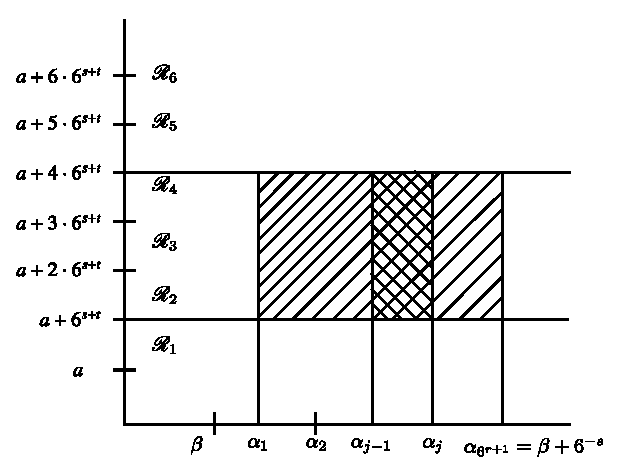
\includegraphics{fig2.eps}
\end{figure}

If\pageoriginale the given sequence is $x_{1}, x_{2}, \ldots$,
construct the points $(x_{1}, 1),\break (x_{2}, 2), (x_{3}, 3), \ldots$. All
these points will be in the ``half strip'' $0 \leq x \leq 1$, $y \geq
0$. To account for our periodic extension of $z(n, \alpha)$, construct
the ``periodic'' set of points $(x_{1} + m_{1}, 1)$, $(x_{2} + m_{2},
2), \ldots$ where $m_{1}, m_{2}, \ldots$ run through the
integers. Then for $n > 0$, $\alpha > 0$, $z(n, \alpha)$ is the number
of points in the rectangle $0 < x \leq \alpha$, $0 \leq y \leq n$. Put 
\begin{align*}
Z = & z(a + 4.6^{s+t}, \beta + 6^{-s}) -z(a + 4.6^{s+t}, \beta + 6^{-s-t-1})\\
& - z(a + 6^{s+t}, \beta + 6^{-s}) + z(a + 6^{s+t}, \beta + 6^{-s-t-1}).
\end{align*}

Write
$$
\alpha_{j} = \beta + j 6^{-s-t-1},
$$
and put
\begin{align*}
z_{j} = & z(a + 4.6^{s+t}, \alpha_{j}) - z(a + 4.6^{s+t}, \alpha_{j-1})\\
 & - z(a + 6^{s+t}, \alpha_{j}) + z(a + 6^{s+t}, \alpha_{j-1}) \qquad (j = 0, 1, 2, \ldots).
\end{align*}

$Z$ is the number of points in the shaded rectangle of the diagram above. Also $z_{j}$ is the number of points in the doubly shaded rectangle. Note that the $z_{j}$ are non-negative integers and that
$$
Z = \sum_{j = 2}^{6^{t+1}} z_{j}.
$$

We shall consider the following two cases separately :
\begin{align*}
 I & : Z > \frac{5}{7} 6^{t}\\
 II & : Z \leq \frac{5}{7} 6^{t}.
\end{align*}

\medskip
\noindent{\textit{Case I.}} $Z > \frac{5}{7} 6^{t}$. For every $n \epsilon \mathfrak{R}_{5}$, $n' \epsilon \mathfrak{R}_{1}$, the rectangle with vertices $(n, \alpha_{j})$, $(n', \alpha_{j})$, $(n, \alpha_{j-1})$, $(n', \alpha_{j-1})$ contains the (doubly shaded) rectangle with vertices $(a + 4.6^{s+t}, \alpha_{j})$, $(a + 6^{s+t}, \alpha_{j})$, $(a + 4.6^{s+t}, \alpha_{j-1})$, $(a + 6^{s+t}, \alpha_{j-1})$, 
and\pageoriginale hence
$$
z(n, \alpha_{j}) - z(n', \alpha_{j}) - z(n, \alpha_{j-1}) + z(n', \alpha_{j-1}) \geq z_{j} (2 \leq j \leq 6^{t+1}).
$$

Therefore
\begin{align*}
D(n, \alpha_{j-1}, \alpha_{j}) - D(n', \alpha_{j-1}, \alpha_{j}) & \geq z_{j} - (n - n')(\alpha_{j} - \alpha_{j-1})\\
 & \geq z_{j} - 5.6^{s+t} 6^{-s-t-1}\\
 & = z_{j} - \frac{5}{6}.
\end{align*}

So
$$
h(\mathfrak{R}_{5}, \mathfrak{R}_{1}, \alpha_{j-1}, \alpha_{j}) \geq z_{j} - \frac{5}{6},
$$
whence
$$
h(\mathfrak{R}_{1}, \mathfrak{R}_{5}, \alpha_{j-1}, \alpha_{j}) \geq \frac{1}{6} z_{j},
$$
since $h(\mathfrak{R}_{1}, \mathfrak{R}_{5}, \alpha_{j-1}, \alpha_{j})$ is non-negative and $z_{j}$ is an integer. On using Lemma 5\ref{chap1:sec5:lem5C}, we obtain
\begin{align*}
& h(\mathscr{T}, \alpha_{j-1}) + h(\mathscr{T}, \alpha_{j})\tag*{$(2 \leq j \leq 6^{t+1})$}\\ 
& \geq \frac{1}{6} z_{j} + \frac{1}{2}(h(\mathfrak{R}_{1}, \alpha_{j-1}) + h(\mathfrak{R}_{1}, \alpha_{j}) + h(\mathfrak{R}_{5}, \alpha_{j-1}) + h(\mathfrak{R}_{5}, \alpha_{j}))
\end{align*}

We shall also require the trivial estimates
\begin{align*}
h(\mathscr{T}, \alpha_{1}) & \geq \frac{1}{2} (h(\mathfrak{R}_{1}, \alpha_{1}) + h(\mathfrak{R}_{5}, \alpha_{1})),\\
h(\mathscr{T}, \alpha_{6^{t+1}}) & \geq \frac{1}{2} (h(\mathfrak{R}_{1}, \alpha_{6^{t+1}}) + h(\mathfrak{R}_{5}, \alpha_{6^{t+1}})),\\
\end{align*}

Taking the sum of all these inequalities, we get
$$
2 \sum_{j=1}^{6^{t+1}} h(\mathscr{T}, \alpha_{j}) \geq \frac{1}{6} \sum_{j=2}^{6^{t+1}} z_{j} + \sum_{j=1}^{6^{t+1}} h(\mathfrak{R}_{1}, \alpha_{j}) + \sum_{j=1}^{6^{t+1}} h(\mathfrak{R}_{5}, \alpha_{j}).
$$\pageoriginale

Note that $\ell (\mathfrak{R}_{1}) \geq 6^{s+t}$ and
\begin{align*}
\sum_{j=1}^{6^{t+1}} h(\mathfrak{R}_{1}, \alpha_{j}) & = \sum_{j=1}^{6^{t+1}} h(\mathfrak{R}_{1}, \beta + j 6^{-s-t-1})\\
& = \sum_{i = 0}^{5} \left(\sum_{\substack{j=1\\j \equiv i(mod 6)}}^{6^{t+1}} h(\mathfrak{R}_{1}, \beta + j 6^{-s-t-1})\right).
\end{align*}

By induction hypothesis, the inner sum here is $\geq 6^{t} \frac{t}{120}$, and our double sum is $\geq 6^{t+1} \frac{t}{120}$. Similarly,
$$
\sum_{j=1}^{6^{t+1}} h(\mathfrak{R}_{5}, \alpha_{j}) \geq \frac{6^{t+1}t}{120}.
$$

Hence 
\begin{align*}
2 \sum_{j = 1}^{6^{t+1}} h(\mathscr{T}, \alpha_{j}) & \geq \frac{1}{6} Z + 2.6^{t+1} \frac{t}{120}\\
& > \frac{1}{6} \frac{5}{7.6} 6^{t+1} + 2.6^{t+1} \frac{t}{120} > \frac{2.6^{t+1}(t+1)}{120}
\end{align*}
i. e.,
$$
\frac{1}{6^{t+1}} \sum_{j = 1}^{6^{t+1}} h(\mathscr{T}, \alpha_{j}) \geq \frac{(t+1)}{120}.
$$

\medskip
\noindent{\textit{Case II.}} $Z \leq \frac{5}{7} 6^{t}$. For every $n \in \mathfrak{R}_{4}$, $n' \in \mathfrak{R}_{2}$, we have
$$
z(n, \alpha_{j}) - z(n', \alpha_{j}) - z(n, \alpha_{j-1}) + z(n', \alpha_{j-1}) \leq z_{j}.
$$

Therefore 
\begin{align*} 
D(n', \alpha_{j-1}, \alpha_{j}) - D(n, \alpha_{j-1}, \alpha_{j}) & \leq -z_{j} + (n - n') (\alpha_{j}, \alpha_{j-1})\\ 
& \geq 6^{s+t} 6^{-s-t-1} - z_{j}\\ 
& = \frac{1}{6} - z_{j},
\end{align*}\pageoriginale 
and we have
$$
h(\mathfrak{R}_{2}, \mathfrak{R}_{4}, \alpha_{j-1}, \alpha_{j}) \geq \frac{1}{6} - z_{j}.
$$

By Lemma 5\ref{chap1:sec5:lem5C},
\begin{align*}
& h(\mathscr{T}, \alpha_{j-1}) + h(\mathscr{T}, \alpha_{j})\tag*{$(2 \leq j \leq 6^{t+1})$}.\\
& \geq \frac{1}{6} z_{j} + \frac{1}{2} (h(\mathfrak{R}_{2}, \alpha_{j-1}) + h(\mathfrak{R}_{2}, \alpha_{j}) + h(\mathfrak{R}_{4}, \alpha_{j-1}) + h(\mathfrak{R}_{4}, \alpha_{j}))
\end{align*}

We also note that the trivial relations
\begin{align*}
h(\mathscr{T}, \alpha_{1}) & \geq \frac{1}{2} (h(\mathfrak{R}_{2}, \alpha_{1}) + h(\mathfrak{R}_{4}, \alpha_{1})),\\
h(\mathscr{T}, \alpha_{6^{t+1}}) & \geq \frac{1}{2} (h(\mathfrak{R}_{2}, \alpha_{6^{t+1}}) + h(\mathfrak{R}_{4}, \alpha_{6^{t+1}})).
\end{align*}

Adding all these inequalities, we obtain
$$
2 \sum_{j=1}^{6^{t+1}} h(\mathscr{T}, \alpha_{j})\geq \frac{1}{6} (6^{t+1} - 1) - Z + \sum_{j=1}^{6^{t+1}} h(\mathfrak{R}_{2}, \alpha_{j}) + \sum_{j=1}^{6^{t+1}} h(\mathfrak{R}_{4}, \alpha_{j}).
$$

Here in Case II, 
$$
\frac{1}{6} (6^{t+1} - 1) - Z \geq \frac{5}{6} 6^{t} - Z \geq \frac{5}{6} 6^{t} - \frac{5}{7} 6^{t} = \frac{5}{42} 6^{t} \geq \frac{2}{120} 6^{t+1}.
$$

Proceeding similarly as in Case I, we finally obtain 
$$
\frac{1}{6^{t+1}} \sum_{j=1}^{6^{t+1}} h(\mathscr{T}, \alpha_{j}) \geq \frac{(t+1)}{120}.
$$

This completes the proof of Lemma 5\ref{chap1:sec5:lem5D}.

\noindent{\em Proof of Theorem 5\ref{chap1:sec5:thm5A}.} First suppose that $N \geq 6^{4}$. Pick $t$ with $6^{t} \leq N  < 6^{t+1}$. Let $\mathscr{T}$ be the interval $0 < n \leq 6^{t}$. Applying Lemma 5\ref{chap1:sec5:lem5D} with $s = 0$.\pageoriginale we get
$$
\frac{1}{6^{t}} \sum_{j=1}^{6^{t}} h(\mathscr{T}, \beta + j 6^{-t}) \geq \frac{t}{120}.
$$

There exists a $\beta$ with
$$
h(\mathscr{T}, \beta) \geq \frac{t}{120}.
$$

So there exists an $n \in \mathscr{T}$ with
\begin{align*}
|D(n, \beta)| \geq \frac{t}{240} & \geq \frac{1}{240} (\log_{6} N - 1)\\
& \geq \frac{1}{320} \log_{6} N > \frac{\log N}{1000}.
\end{align*}

Hence
$$
\triangle(n) > \frac{\log N}{1000},
$$
with $1 \leq n \leq 6^{t} \leq N$. On the other hand, if $N < 6^{4}$, then $\triangle(1) \geq |D(1, \frac{1}{2})| \geq \frac{1}{2} > \frac{\log N}{1000}$. The proof of Theorem 5\ref{chap1:sec5:thm5A} is complete.

\section{A question of Erd\"{o}s}\label{chap1:sec6}

It was known since Ehrenfest result (see \S\ \ref{chap1:sec2}), that $\triangle(n)$ is bounded. Recall that $\triangle(n) = \sup\limits_{I \subseteq U} |D(n, I)|$. P.Erd\"os \cite{5} asked the following question:

\medskip
\noindent{\textit{Does there always exist an interval $I \subseteq U$ such that $D(n, I)$ is un-bounded?}}

This question was answered, in the affirmative, by W. M. Schmidt \cite{21}.

A stronger result is
\begin{theorem}\label{chap1:sec6:thm6A}
There always exists an $\alpha \epsilon U$ with
$$
\mathop{\lim \sup}_{n \to \infty} \frac{|D(n, \alpha)|}{\log n} > \frac{1}{2000}.
$$
\end{theorem}

($\alpha$ depends on the sequence $x_{1}, x_{2}, \ldots$ ).

The proof of Theorem 6\ref{chap1:sec6:thm6A} depends on Lemma 5\ref{chap1:sec5:lem5D} and the following simple

\begin{lemma}\label{chap1:sec6:lem6B}
Suppose that $0 < \epsilon < n$ and $\alpha \in U$. Then there exists a closed subinterval $I$ of $U$ containing $\alpha$ such that $|I| = \epsilon/n$ and 
\begin{equation*}
|D(n, \beta)| \geq |D(n, \alpha)| - \epsilon\tag{6.1}\label{chap1:sec6:eq6.1}
\end{equation*}
for every $\beta \epsilon I$.
\end{lemma}\pageoriginale

\begin{proof}
 We distinguish three cases.
 \end{proof}


\noindent{\textbf{Case I.}} $|D(n, \alpha)| \leq \epsilon$. The lemma follows trivially, since now the right hand side of $(6.1)$ is $\leq 0$.

\medskip
\noindent{\textbf{Case II.}} $D(n, \alpha)> \epsilon$. In this case we have
$$
n - n\alpha \geq z(n, \alpha) - n\alpha = D(n, \alpha) > \epsilon,
$$
whence
$$
\alpha < 1 - \frac{\epsilon}{n}.
$$

Let $I$ be the interval
$$
\alpha \leq \beta \leq \alpha + \frac{\epsilon}{n}.
$$

Observe that $I \subseteq U$ with $|I| = \frac{\epsilon}{n}$, and for $\beta \in I$ we have
\begin{align*}
|D(n, \beta)| & \geq z(n, \beta) - n\beta\\
& \geq z(n, \alpha) -n\alpha + n(\alpha - \beta)\\
& \geq |D(n, \alpha)| - \epsilon.
\end{align*}

\medskip
\noindent{\textbf{Case III.}} $D(n, \alpha) < - \epsilon$. We now have
$$
n \alpha \geq n\alpha -z(n, \alpha) = -D(n, \alpha) > \epsilon,
$$
whence
$$
\alpha > \frac{\epsilon}{n}.
$$

We take $I$ to be the interval 
$$
\alpha - \frac{\epsilon}{n} \leq \beta \leq \alpha.
$$

Then $I \subseteq U$ with $|I| = \frac{\epsilon}{n}$, and for $\beta \in I$,
\begin{align*}
|D(n, \beta)| & \geq n\beta -z(n, \beta)\\
& \geq n\alpha -z(n, \alpha) -n(\alpha - \beta)\\
& \geq |D(n, \alpha)| - \epsilon.
\end{align*}\pageoriginale

\medskip
\noindent{\textit{Proof of Theorem 6\ref{chap1:sec6:thm6A}.}} It is sufficient to proof the following:
{\em There exists a nested sequence $I_{1} \supseteq \ldots \supseteq I_{m} \supseteq \ldots$ of closed intervals and positive integers $n_{1} < \ldots < n_{m} < \ldots$, such that for every} $\beta \in I_{m}$,
$$
|D(n_{m}, \beta)| \geq \frac{1}{2000} \log n_{m}.
$$

(Since $\bigcap\limits_{m=I}^{\infty} I_{m} \neq \phi$ choose $\alpha \epsilon \bigcap\limits_{m=I}^{\infty} I_{m}$. Then $|D(n_{m}, \alpha)| \geq \frac{\log n_{m}}{2000}$ for every $m$.

So Theorem 6\ref{chap1:sec6:thm6A} follows).

The proof is by induction on $m$. If $m=1$, take $I_{1} = U$, $n_{1} = 1$, and the desired inequality holds trivially. Suppose that $I_{1}, \ldots, I_{m-1}$ and $n_{1}, \ldots, n_{m-1}$ are already constructed. Let $I'_{m-1}$ by the subinterval of $I_{m-1}$ with $|I'_{m-1}| = \frac{1}{2} |I_{m-1}|$ and with the same midpoint as $I_{m-1}$. Choose $s$ so large that
\begin{equation*}
6^{-s} \leq |I'_{m-1}|.\tag{6.2}\label{chap1:sec6:eq6.2}
\end{equation*}

Further choose $t$ so large that
\begin{equation*}
t > s, t > 250 n_{m-1}.\tag{6.3}\label{chap1:sec6:eq6.3}
\end{equation*}

Let $\beta$ be the left and points of $I'_{m-1}$. Let $\mathscr{T}$ be the interval of integers $n$ with $0 < n \leq 6^{s+t}$. We now apply Lemma 5\ref{chap1:sec5:lem5D} and obtain
$$
\frac{1}{6^{t}} \sum_{j=1}^{6^{t}} h(\mathscr{T}, \beta + j 6^{-s-t}) > \frac{t}{120}.
$$

By (\ref{chap1:sec6:eq6.2}),
$$
\beta + j 6^{-s-t} \in I'_{m-1} \qquad (1 \leq j \leq 6^{t}).
$$

Hence\pageoriginale there exists an $\alpha \in I'_{m-1}$ with
$$
h(\mathscr{T}, \alpha) > \frac{t}{120}.
$$

There exists an $n \in \mathscr{T}$, $0 < n \leq 6^{s+t}$, with
$$
|D(n, \alpha)| > \frac{t}{240}.
$$

Now $\alpha$ lies in the interior of $I_{m-1}$. Hence if we choose $\epsilon > 0$ sufficiently small and apply Lemma 6\ref{chap1:sec6:lem6B}, we see the existence of a closed subinterval $I_{m}$ of $I_{m-1}$ such that
\begin{equation*}
 |D(n, \beta)| > \frac{t}{250},\tag{6.4}\label{chap1:sec6:eq6.4}
\end{equation*}
for every $\beta \epsilon I_{m}$. Since $|D(n, \beta)| \leq n$, (\ref{chap1:sec6:eq6.3}) and (\ref{chap1:sec6:eq6.4}) yield
$$
n > \frac{t}{250} > n_{m-1}.
$$

Set $n_{m} = n$. It follows from (\ref{chap1:sec6:eq6.3}) and (\ref{chap1:sec6:eq6.4}), that for every $\beta \in I_{m}$
$$
|D(n_{m}, \beta)| > \frac{t}{250} > \frac{s+t}{500} \geq \frac{\log_{6} n_{m}}{500} \geq \frac{\log n_{m}}{2000}.
$$

This completes our inductive construction.

\begin{theorem}\label{chap1:sec6:thm6C}
 For almost every $\alpha$,
$$
\mathop{\lim \sup}_{n \to \infty} \frac{D(n, \alpha)}{\log \log n} > \frac{1}{2000}.
$$
\end{theorem}

This is stronger than in a paper by W. M. Schmidt \cite{21}. It is an
open problem whether $\log \log n$ may be replaced by a faster
increasing function, perhaps even by $\log n$. 

\begin{proof} 
For $k = 1, 2, \ldots,$ the intervals $\frac{u}{k!} \leq x \leq
\frac{(u+1)}{k!}$ with $u = 0, 1, \ldots,\break (k! - 1)$ will be called
     {\em interval of order} $k$. Given any interval $I$, the
     subinterval with the same midpoint as $I$ and with length
     $\frac{1}{2}|I|$ will be denoted by $I'$. 
\end{proof}

Let\pageoriginale $k$ be a fixed large integer; say $k > k_{0} =
100$. Put $N = N(K) = k!$. Let $I_{k-1}$ be an interval of order
$k-1$. Choose $s$ with $6^{s-1} \leq 2(k-1)! \leq 6^{s}$. Let $t$ be
such that $6^{s+t} \leq N(k) < 6^{s+t+1}$. Then $t \geq 1$ in view of
$k > 100 > 72$. Let $\beta$ be the left end point of
$I'_{k-1}$. Denote by $\mathscr{T}$ the interval $0 < n \leq
6^{s+t}$. By Lemma 5\ref{chap1:sec5:lem5D}, we obtain 
$$
\frac{1}{6^{t}} \sum_{j=1}^{6^{t}} h(\mathscr{T}, \beta + j 6^{-s-t}) \geq \frac{t}{120}.
$$

Observe that $\beta + j 6^{-s-t} \in I'_{k-1} (0 < j \leq 6^{t})$, since $j 6^{-s-t} \leq 6^{-s} \leq \frac{1}{2(k-1)!}$. Hence there is a $\beta_{0} \in I'_{k-1}$ and an integer $n$, $0 < n \leq 6^{s+t} \leq N$, with
$$
|D(n, \beta_{0})| \geq \frac{t}{240}.
$$

By Lemma 6\ref{chap1:sec6:lem6B} with $\epsilon = 2$, there is an interval $I$ of length $\frac{\epsilon}{n} \geq \frac{2}{k!}$ containing $\beta_{0}$, such that
$$
|D(n, \alpha)| \geq \frac{t}{240} - 2,
$$
for every $\alpha \in I$. Since $k$ is large, $I \leq I_{k-1}$. Now $|I| \leq \frac{2}{k!}$, and therefore $I$ and a fortiori $I_{k-1}$ contains a subinterval $I_{k}$ of order $k$ having 
$$
|D(n, \alpha)| \geq \frac{t}{240} - 2,
$$
for every $\alpha \in I_{k}$. Now
$$
6^{t} = 6^{s+t+1-s-1} \geq N(k) \frac{1}{6^{2} . 2(k-1)!} = \frac{k}{72}
$$
and
$$
\log N(k) \leq k \log k \leq k^{2}.
$$

Hence for every $\alpha \in I_{k}$,
\begin{align*}
|D(n, \alpha)| \geq \frac{1}{240} \log_{6} (\frac{k}{72}) - 2 > \frac{1}{1000} \log k & \geq \frac{1}{2000} \log \log N(k)\tag{6.5}\label{chap1:sec6:eq6.5}\\
& \geq \frac{1}{2000} \log \log n.
\end{align*}

For\pageoriginale every interval $I_{k-1}$ of order $k-1 (\geq k_{0} - 1)$, we may select a subinterval $I_{k}$ of order $k$ with the property (\ref{chap1:sec6:eq6.5}). Denote the union of the intervals $I_{k}$ so obtained by $E(k)$. Let $\alpha$ be such that it lies in infinitely many of the sets $E(k_{0}), E(k_{0} + 1), \ldots$. Then the inequality
$$
|D(n, \alpha)| \geq \frac{1}{2000} \log \log n
$$
holds for infinitely many $n$. Hence Theorem 6\ref{chap1:sec6:thm6C} is proved if we can show that almost every $\alpha$ lies in infinitely many of the sets $E(k_{0}), E(k_{0} + 1), \ldots$.

For every natural number $K \geq k_{0}$, let $T_{K}$ be the complement of $\bigcup\limits_{k \geq K} E(k)$. It is sufficient to prove that $\mu (T_{K}) = 0$ for every $K$ ($\mu$ denotes the Lebesgue measure). But this is so, since
$$
\mu (T_{K}) = \prod_{k=K}^{\infty} (1-\mu(E_{k}))=\prod_{k=K}^{\infty}(1-\frac{1}{k}) = 0.
$$

This proves Theorem 6\ref{chap1:sec6:thm6C}.

\section{The Scarcity of Intervals With Bounded Error}\label{chap1:sec7} 

Recall that for $\alpha \in U$, $D(n, \alpha) = z(n, \alpha)-n\alpha$. Put
$$
E(\alpha) = \sup_{n}|D(n, \alpha)|,
$$
where the supremum is taken over all positive integers $n$. For every non-negative $\mathcal{K}$, let $S(\mathcal{K})$ be the set of all those $\alpha \in U$ which have $E(\alpha) \leq \mathcal{K}$.

Let $S(\infty)$ consist of $\alpha$ in $U$ with $E(\alpha) < \infty$. Clearly,
$$
S(\infty) = \bigcap\limits_{\mathcal{K}=0}^{\infty} S(\mathcal{K}).
$$

We shall prove that $S(\infty)$ is at most countable.

The {\em derivative} of a set $S$ of real numbers is the collection of the limit points of S. It will be denoted by $S^{(1)}$. Define inductively
$$
S^{(d)} = (S^{(d-1)})^{(1)} \qquad(d = 2, 3, \ldots).
$$

For\pageoriginale convince, we shall write $S^{(0)}$ for $S$.

\begin{theorem}\label{chap1:sec7:thm7A}
(W. M. Schmidt \cite{24}) Suppose that $d > 4\mathcal{K}$. Then
$$
(S(\mathcal{K}))^{(d)} = \phi,
$$
i. e., the empty set.
\end{theorem}

In view of the following lemma, Theorem 7\ref{chap1:sec7:thm7A} implies that $S(\infty)$ is at most countable.

\begin{lemma}\label{chap1:sec7:thm7B}
Suppose that $S$ is a set of real numbers having $S(d) = \phi$ for some $d$. Then $S$ is at most countable and is nowhere dense.
\end{lemma}

\begin{proof} 
We claim that for any set $A$ of real numbers, the set theoretic difference $B = A - A^{(1)}$ is at most countable. Denote by $\mathfrak{S}$ the collection of all the open intervals $N$ with rational end points. Note that $\mathfrak{S}$ is countable. Further observe that for $x$ in $B$, there exists an interval $N_{x}$ of $\mathfrak{S}$ with $N_{x} \cap B = x$. For distinct $x_{1}, x_{2}$ in $B$, the intervals $N_{x_{1}}, N_{x_{2}}$ are distinct. This shows that $B$ is countable, since $\mathfrak{S}$ is so.
\end{proof}

We have $A = (A-A^{(1)}) \cup (A \cap A^{(1)})$. Hence if $A^{(1)}$ is at most countable, then so is $A$. Hence if $S^{(d)} = \phi$, then $S$ is at most countable. 

Now suppose that $A^{(1)}$ is nowhere dense. Then every interval $I$ contains a closed subinterval $J_{1}$ with $J_{1} \cap A^{(1)} = \phi$. Then $J_{1} \cap A$ is finite. Thus there is a subinterval $J$ of $J_{1}$ with $J \cap A = \phi$. Thus $A$ is nowhere dense. More generally, if $A^{(d)}$ is nowhere dense, then so is $A$. If $S^{(d)} = \phi$, then $S$ is nowhere dense.

\begin{coro*}
  For every non-negative $\mathcal{K}$, $S(\mathcal{K})$ is at most countable  and is nowhere dense. The set $S(\infty)$ is at most countable.
\end{coro*}

For $I \subseteq U$, set
\begin{align*}
  D(n, I) & = z(n, I) - n|I|,\\
  E(I) & = \sup_{n} |D(n, I)|.
\end{align*}\pageoriginale

We may call $E(I)$ the {\em error} of I.

\begin{theorem}[$^*$]\label{chap1:sec7:thm7C}
(W. M. Schmidt \cite{26}.) The lengths of all the intervals $I$ with finite error $E(I)$ form at most a countable set\footnote{see remark on page \pageref{55}.}.
\end{theorem}

The above Theorem does not give any information about the cardinality of the set of intervals $I$ with $E(I) < \infty$. It has the power of continuum in the following case.

\begin{theorem}[$^*$]\label{chap1:sec7:thm7D}
Let $\alpha$ be an irrational number. Consider the sequence
$$
\{\alpha\}, \{2\alpha\}, \ldots .
$$
\end{theorem}

Then $E(I)$ is finite if and only if $I = \{k\alpha\}$ for some non-zero integer $k$. 

The ``if'' part is due to $A$. Ostrowski \cite{17}. The ``only if'' part was shown by H. Kesten \cite{11}\footnote{Addded June 1976. H.Furstenberg, H. Keynes and L. Shapiro (Prime flows in topological dynamics, Israel J. Math, 14(1) (1973), 26-38) and G. Hal\'{a}sz (Remarks on the remainder in Birkhoff Ergodic Theorem (preprint)) proved this with ergodic theorey.}.

A proof of the ``if'' part is as follows. More generally, we shall consider the sequence
$$
\{\alpha + \beta\}, \{2\alpha + \beta\}, \ldots .
$$

Because of the arbitrary parameter $\beta$, it will be sufficient to deal with the case when $I$ is of the type $0 \leq x < \{k \alpha\}$. We may assume that $0 < \{k \alpha\} < 1$. Further we may assume that $k > 0$ : For if $k < 0$, put $k=-k'$, $k' > 0$. Then the length of the complement $I'$ of $I$ in $U$ is equal to $\{k' \alpha\}$, since $\{k\alpha\} + \{k' \alpha\} = 1$. We have $E(I) = E(I')$, so that $E(I)$ is finite if $E(I')$ is finite,\pageoriginale and in particular $E(I)$ is finite if the `if' part of the theorem is true for $k' > 0$.

Consider the $k$ sequence
\begin{equation*}
 \begin{matrix}
  \{\alpha + \beta\},  & \{(k+1)\alpha + \beta\}, & \ldots,\\
  \{2\alpha + \beta\}, & \{(k+2)\alpha + \beta\}, & \ldots,\\
  \hdotsfor{3}\\
  \{k\alpha + \beta\}, & \{2k\alpha + \beta\}, & \ldots .
 \end{matrix}
\end{equation*}

It is sufficient to prove that $E(I)$ is finite for each of these sequences. In each of these sequences, the common differences of the arithmetic progression is $k \alpha$. Since $|I| = \{k \alpha\}$, we may replace $\alpha$ by $k \alpha$ and see that it will suffice to prove the assertion in the special case when $|I| = \{\alpha\}$, i. e. the special case $k = 1$. Thus the problem reduces to showing that $E(I)$, with $I$ : $0 \leq x < \alpha$, is finite for the sequence
$$
\{\alpha + \beta\}, \{2\alpha + \beta\}, \ldots .
$$

Observe that
\begin{align*}
z(n, I) & = \text{ the number of }k, 1 \leq k \leq n, \text{ with } \{k \alpha + \beta\} < \alpha\\
& = \text{ the number of integers } m \text{ and }k, 1 \leq k \leq n, \text{ satisfying the}\\ 
& \tag*{inequality } 
\end{align*}
$$
0 \leq k\alpha + \beta -m < \alpha.
$$

Any $m$ satisfying this inequality with $1 \leq k \leq n$ must satisfy
$$
\beta < m \leq n\alpha + \beta.
$$

For every $m$, there exists a unique integer $k$ satisfying the first inequality.

Moreover if $m$ satisfies the second inequality, then this integer $k$ satisfies $1 \leq k \leq n$. Hence $z(n, I)$ is equal to the number of integers $m$ satisfying the second inequality, and $|z(n, I) - n\alpha| \leq 1$.

Therefore\pageoriginale $|D(n. I)| \leq 1$ for every integer $n$, and $E(I) \leq 1$.

This proves the `if' part of Theorem 7\ref{chap1:sec7:thm7D}. The more difficult `only if' part will not be proved here.

Denote by $U^{0}$ the open unit interval $0 < x < 1$. BY a {\em neighbourhood}, we shall always mean an open interval contained in $U^{0}$. For the proof of Theorem 7\ref{chap1:sec7:thm7A}, we shall need several lemmas.

\begin{lemma}\label{chap1:sec7:lem7E}
Let $\alpha \in U^{0}$ and $\epsilon > 0$ be given. Then there exists a neighbourhood $A$ of $\alpha$, and an integer $p$, such that for any $\beta \in A$ and for any interval $\mathscr{T}$ of integers with $\ell (\mathscr{T}) \geq p$,
$$
h(\mathscr{T}, \beta) \geq \frac{1}{2} - \epsilon.
$$
\end{lemma}

\begin{proof} 
Assume at first that $0 < \alpha \leq \frac{1}{2}$. Put
$$
p = \left[\frac{1}{\alpha}\right] + 1.
$$

Consider the numbers 
$$
\alpha, 2\alpha, \ldots, p\alpha.
$$

Every number $\psi$ with $\frac{\alpha}{2} \leq \psi \leq (p + \frac{1}{2})\alpha$ has a distance $\leq \frac{\alpha}{2}$ from (at least) one of these $p$ numbers. Hence it has a distance $\leq \frac{1}{4}$. Thus for every $\psi$ with $\frac{\alpha}{2} \leq \psi \leq (p + \frac{1}{2})\alpha$, there is an integer $n$, $1 \leq n \leq p$, such that $|n\alpha - \psi| \leq \frac{1}{4}$.
\end{proof}

Since $\frac{\alpha}{2} \leq \psi \leq (p + \frac{1}{2})\alpha$ has length $p \alpha > 1$, the translations of this interval by integers cover the real line. Therefore for any real number $\psi$, there exist integers $n$, $m$ with $0 < n \leq p$ and $|n \alpha - m - \psi| \leq \frac{1}{4}$. Further the 
restriction $0 < \alpha \leq \frac{1}{2}$ can be removed, since for $\frac{1}{2} < \alpha \leq 1$, there exist integers $n$, $m'$ such that $0 < n \leq p$ and $|n(1 - \alpha) - m' + \psi| \leq \frac{1}{4}$, i.e. $|n\alpha - m - \psi| \leq \frac{1}{4}$, with $m = n-m'$.

Let $A$ consist of $\beta \in U^{0}$ with $p|\beta - \alpha| < \frac{\epsilon}{2}$. For every real number $\psi$, there are integers $n$, $m$, $0 < n \leq p$, such that $|n \beta - m - \psi| < \frac{1}{4} + \frac{\epsilon}{2}$ holds for all $\beta \in A$, since $|n\alpha - m - \psi| \leq \frac{1}{4}$ and $0 < n \leq p$, implies that $|n \beta - m - \psi| < \frac{1}{4} + \frac{\epsilon}{2}$ for $\beta \in A$.\pageoriginale Now since $\psi$ is arbitrary, we see that for every $\psi$, there are integers $n$, $m$, $0 < n \leq p$, having $0 < n\beta - m \psi < \frac{1}{2} + \epsilon$ for every $\beta \in A$. {\em Hence for every interval $\mathscr{T}$ with $\ell (\mathscr{T}) \geq p$, every $\beta \in A$ and every $\psi$, there are integers $n, m$ with $n \in \mathscr{T}$ and}
$$
0 < n\beta - m - \psi < \frac{1}{2} + \epsilon.
$$

For $\beta \in A$ and an interval $\mathscr{T}$ with $\ell (\mathscr{T}) \geq p$, choose integers $n \in \mathscr{T}$ and $m$ such that
\begin{equation*}
0 < n\beta - m + g^{-} (\mathscr{T}, \beta) < \frac{1}{2} + \epsilon.\tag{7.1} \label{chap1:sec7:eq7.1}
\end{equation*}

Then
$$
z(n, \beta) = D(n, \beta) + n\beta \geq g^{-} (n, \beta) + n\beta > m.
$$

Therefore
\begin{equation*}
z(n, \beta) \geq m+1.\tag{7.2} \label{chap1:sec7:eq7.2}
\end{equation*}

Combining (\ref{chap1:sec7:eq7.1}) and (\ref{chap1:sec7:eq7.2}), we obtain
\begin{align*}
h(\mathscr{T}, \beta) & = g^{+} (\mathscr{T}, \beta) - g^{-}(\mathscr{T}, \beta)\\
 & \geq D(n, \beta) - g^{-} (\mathscr{T}, \beta)\\
 & = z(n, \beta) - n\beta - g^{-} (\mathscr{T}, \beta)\\
 & > m + 1 - m - \frac{1}{2} - \epsilon\\
 & = \frac{1}{2} - \epsilon.
\end{align*}

This is true for every $\beta \in A$. Lemma 7\ref{chap1:sec7:lem7E} is proven.

\begin{lemma}\label{chap1:sec7:lem7F}
Suppose that $0 < \epsilon < 1$ and $q \geq 1$ is an integer. Suppose that $\alpha, \beta \in U^{0}$ with $0 < |\alpha - \beta| < \frac{\epsilon}{8q}$. Then there is an integer $p$ and there are neighbourhoods $A$ of $\alpha$, $B$ of $\beta$ with the following property: If $\mathscr{T}$ is an interval with $\ell (\mathscr{T}) \leq p$ and if $\gamma \in A$, $\delta \in B$, then there exist subintervals $\mathfrak{R}, \mathfrak{R}'$\pageoriginale of $\mathscr{T}$ with $\ell(\mathfrak{R}) = \ell(\mathfrak{R}') = q$ and
$$
g^{-} (\mathscr{R}, \gamma, \delta) - g^{+} (\mathscr{R}', \gamma, \delta) > 1 - \epsilon.
$$
\end{lemma}

\begin{proof} 
We may assume that $\alpha < \beta$. Put $p_{0} = \frac{1}{\beta - \alpha} + 1$. By an argument as in the proof of Lemma 7\ref{chap1:sec7:lem7E}, one sees that for every real number $\psi$, there exist integers $n$, $m$, $1 \leq n \leq p_{0}$, such that
$$
|n(\beta - \alpha) - m -\psi| \leq \frac{1}{2} |\beta - \alpha| < \frac{\epsilon}{8}.
$$

Let A consist of $\gamma \in U^{0}$ with
$$
|\gamma - \alpha| \max (q, p_{0}) < \frac{\epsilon}{16},
$$
and B of $\delta \in U^{0}$ with
$$
|\delta - \beta| \max (q, p_{0}) < \frac{\epsilon}{16}. 
$$
\end{proof}

Then for every $\gamma \in A$ and $\delta \in B$, and for every $\psi$, there are integers $n$, $m$ with $0 < n \leq p_{0}$ and
$$
|n(\delta - \gamma) - m - \psi| < \frac{\epsilon}{4}.
$$ 

Now since $\psi$ is arbitrary, it follows that for every $\gamma \in A$, every $\delta \in B$ and every $\psi$, there exist integers $n$, $m$, $0 < n \leq p_{0}$, with
$$
0 < n(\delta - \gamma) - m - \psi < \frac{\epsilon}{2}.
$$

Here the condition $0 < n \leq p_{0}$ may be replaced by $n \in \mathscr{T}$, where $\mathscr{T}$ is a given interval with $\ell (\mathscr{T}) \geq p_{0}$.

Suppose that $\mathscr{T}_{\circ}$ is any interval with $\ell (\mathscr{T}_{\circ}) \leq p_{0}$. Let $\gamma \in A$ and $\delta \in B$ be fixed. Choose $n'_{0} \in \mathscr{T}_{\circ}$ with
$$
g^{-} (\mathscr{T}_{\circ}, \gamma, \delta) = D(n'_{0}, \gamma, \delta).
$$

Choose integers $n_{0} \in \mathscr{T}_{\circ}$ and $m$ such that
\begin{equation*}
0 < n_{0} (\delta - \gamma)- m + g^{-} (\mathscr{T}_{0}, \gamma, \delta) < \frac{\epsilon}{2}.\tag{7.3}\label{chap1:sec7:eq7.3}
\end{equation*}

Then
\begin{align*}
z(n_{0}, \delta) - z(n_{0}, \gamma) & = D(n_{0}, \gamma, \delta) + n_{0} (\delta - \gamma)\\
& \geq g^{-} (\mathscr{T}_{\circ}, \gamma, \delta) + n_{0} (\delta - \gamma)\\
& > m.\\
\end{align*}

Therefore\pageoriginale
\begin{equation*}
z(n_{0}, \delta) - z(n_{0}, \alpha) \geq m+1\tag{7.4}\label{chap1:sec7:eq7.4}
\end{equation*}

Combining (\ref{chap1:sec7:eq7.3}) and (\ref{chap1:sec7:eq7.4}), we obtain
\begin{align*}
D(n_{0}, \gamma, \delta) -D(n'_{0}, \gamma, \delta) & \geq m+1 -n_{0} (\delta - \gamma) - g^{-} (\mathscr{T}_{\circ}, \gamma, \delta)\\
& > m + 1 - m - \frac{\epsilon}{2}\\
 & = 1 - \frac{\epsilon}{2}\tag{7.5}\label{chap1:sec7:eq7.5}
\end{align*}

Now put
$$
p = p_{0} + 2q.
$$

Suppose that $\mathscr{T}$ is an interval with $\ell (\mathscr{T}) \geq p$. Let $\mathscr{T}_{\circ}$ be the interval obtained from $\mathscr{T}$ by cutting off segments of length $q$ on either side. Then clearly $\ell (\mathscr{T}_{0}) \geq p_{0}$. Hence there exist integers $n_{0}$, $n'_{0} \in \mathscr{T}_{\circ}$ satisfying (\ref{chap1:sec7:eq7.5}). Set
$$
\mathfrak{R} : n_{0} < n \leq n_{0} + q \text{ and }\mathfrak{R}' : n'_{0} - q < n' \leq n'_{0}.
$$

It is clear that 
$$
\ell (\mathfrak{R}) = \ell(\mathfrak{R}') = q \text{ and } \mathfrak{R}, \mathfrak{R}' \subseteq \mathscr{T}.
$$

For every $n \in \mathfrak{R}$ we have
\begin{align*}
D(n, \gamma, \delta) - D(n_{0}, \gamma, \delta) & \geq -(n - n_{0}) (\delta - \gamma)\\
& \geq -q (\delta - \alpha) > - \frac{\epsilon}{4},\tag{7.6}\label{chap1:sec7:eq7.6}
\end{align*}
since $\gamma \in A$, $\delta \in B$ has
$$
|\gamma - \delta| \leq |\gamma - \alpha| + |\alpha - \beta| + |\beta - \delta| < \frac{\epsilon}{16q} + \frac{\epsilon}{8q} + \frac{\epsilon}{16q} = \frac{\epsilon}{4q}.
$$

Similarly, for every $n' \in \mathfrak{R}'$, we have
\begin{equation*}
D(n'_{0}, \gamma, \delta) - D(n', \gamma, \delta) > - \frac{\epsilon}{4}.\tag{7.7}\label{chap1:sec7:eq7.7}
\end{equation*}

Adding (\ref{chap1:sec7:eq7.5}), (\ref{chap1:sec7:eq7.6}) and (\ref{chap1:sec7:eq7.7}), we get 
$$
D(n, \gamma, \alpha) - D(n', \gamma, \delta) > 1 - \in.
$$\pageoriginale

This holds for every $n \in \mathfrak{R}$ and every $n' \in
\mathfrak{R}'$. Lemma 7\ref{chap1:sec7:lem7F} follows immediately

\begin{lemma}\label{chap1:sec7:lem7G}
Suppose that $\theta_{1}, \ldots, \theta_{t} \in U^{0}$ and
belong to the derivative $R^{(1)}$ of some set $R$ of real
numbers. Let $D_{1}, \ldots, D_{t}$ be respective neighbourhoods of
$\theta_{1}, \ldots, \theta_{t}$. Let $\in > 0$ and an integer
$q \geq 1$ be given. Then there exist numbers $\alpha_{1}, \beta_{1},
\ldots, \alpha_{t}, \beta_{t}$ of R such that $\alpha_{1}, \beta_{1}
\in D_{1}, \ldots, \alpha_{t}, \beta_{t} \in D_{t}$, there
exist neighbourhoods $A_{1}, B_{1}, \ldots, A_{t}, B_{t}$ of
$\alpha_{1},\break \beta_{1}, \ldots, \alpha_{t}, \beta_{t}$, respectively,
with $A_{1}, B_{1} \subseteq D_{1}, \ldots, A_{t}, B_{t} \subseteq
D_{t}$, and there exists an integer $r$ with the following property :
If $\mathscr{T}.\mathscr{T}'$ are intervals with $\ell
(\mathscr{T}) \geq r$, $\ell (\mathscr{T}') \geq r$ and if
$\gamma_{1}, \delta_{1}, \ldots, \gamma_{t}, \delta_{t}$ lie in
$A_{1}, B_{1}, \ldots$, $A_{t}, B_{t}$, respectively, then there are
subintervals $\mathfrak{R} \subseteq \mathscr{T}, \mathfrak{R}'
\subseteq \mathscr{T}$ with $\ell (\mathfrak{R}) = \ell
(\mathfrak{R}') = q$ and
$$
h(\mathfrak{R}, \mathfrak{R}', \gamma_{i}, \delta_{i}) > 1 - \in
\qquad (i = 1, \ldots, t).
$$
\end{lemma}

We shall apply this lemma with $\mathscr{T} = \mathscr{T}'$, but
generality is necessary to carry out the inductive proof.

\begin{proof} 
Suppose at first that $t =
1$. Then $\theta_{1} \in R^{(1)}$, a neighbourhood $D_{1}$ of
$\theta_{1}$, $\in > 0$ and an integer $q \geq 1$ are given. We
may suppose that $0 < \in < 1$. Since $\theta_{1} \in
R^{(1)}$, there exist elements $\alpha_{1}, \beta_{1} \in R \cap
D_{1}$ with $0 < |\alpha_{1} - \beta_{1}| < \frac{\epsilon}{8q}$. We
now apply Lemma 7\ref{chap1:sec7:lem7F}. There exist neighbourhoods $A_{1}$ of
$\alpha_{1}, B_{1}$ of $\beta_{1}$, and an integer $p$ as follows: If
$\mathscr{T}$ is an interval with $\ell(\mathscr{T}) \geq p$ and if
$\gamma_{1} \in A_{1}$, $\delta_{1} \in B_{1}$, then there
exist intervals $\mathfrak{R}_{1}, \mathfrak{R}_{2} \subseteq
\mathscr{T}$ such that $\ell (\mathfrak{R}_{1}) = \ell
(\mathfrak{R}_{2}) = q$ and
\begin{equation*}
g^{-} (\mathfrak{R}_{1}, \gamma_{1}, \delta_{1}) - g^{+}
(\mathfrak{R}_{2}, \gamma_{1}, \delta_{1}) > 1 - \epsilon\tag{7.8}\label{chap1:sec7:eq7.8}
\end{equation*}

We may choose $A_{1}$, $B_{1}$ such that $A_{1}$, $B_{1} \subseteq
D_{1}$.
\end{proof}

Let\pageoriginale $\mathscr{T}'$ be another interval with $l(\mathscr{T}') \geq p$. By applying Lemma 7\ref{chap1:sec7:lem7F} again, we conclude that these exist $\mathfrak{R}'_{1}, \mathfrak{R}'_{2} \subseteq \mathscr{T}'$ with $\ell (\mathfrak{R}'_{1}) = \ell (\mathfrak{R}'_{2}) = q$ and 
\begin{equation*}
g^{-} (\mathfrak{R}'_{1}, \gamma_{1}, \delta_{1}) - g^{+} (\mathfrak{R}'_{2}, \gamma_{1}, \delta_{1}) > 1 - \epsilon.\tag{7.9}\label{chap1:sec7:eq7.9}
\end{equation*}

From (\ref{chap1:sec7:eq7.8}) and (\ref{chap1:sec7:eq7.9}) it follows that either
$$
g^{-} (\mathfrak{R}_{1}, \gamma_{1}, \delta_{1}) - g^{+} (\mathfrak{R}'_{2}, \gamma_{1}, \delta_{1}) > 1 - \epsilon
$$
or 
$$
g^{-} (\mathfrak{R}'_{1}, \gamma_{1}, \delta_{1}) - g^{+} (\mathfrak{R}_{2}, \gamma_{1}, \delta_{1}) > 1 - \epsilon.
$$

Therefore 
$$
\text{ either } h(\mathfrak{R}_{1}, \mathfrak{R}'_{2}, \gamma_{1}, \delta_{1}) > 1 - \epsilon \text{ or } h(\mathfrak{R}_{2}, \mathfrak{R}'_{1}, \gamma, \delta) > 1 - \epsilon.
$$

In the first case put $\mathfrak{R} = \mathfrak{R}_{1}, \mathfrak{R}' = \mathfrak{R}'_{2}$, and in the second case out $\mathfrak{R} = \mathfrak{R}_{2}, \mathfrak{R}' = \mathfrak{R}'_{1}$.

Hence
$$
h(\mathfrak{R}, \mathfrak{R}', \gamma_{1}, \delta_{1}) > 1 - \epsilon.
$$

Thus the lemma is proved for $t = 1$ with $r^{(1)} = p$.

We now shall do the inductive step from $t-1$ to $t$. Suppose we are given $\theta_{1}, \ldots, \theta_{t} \in R^{(1)}$ with respective neighbourhoods $D_{1}, \ldots, D_{t}$, $\epsilon > 0$ and an integer $q \geq 1$. By induction hypothesis there exist $\alpha_{1}, \beta_{1}, \ldots, \alpha_{t-1}, \beta_{t-1}$ and an integer $r^{(t-1)}$ satisfying the conclusions of the lemma. Therefore if $\mathscr{T}$ and $\mathscr{T}'$ are intervals with $\ell (\mathscr{T})$, $\ell(\mathscr{T}') \geq r^{(t-1)}$ and if $\gamma_{1} \in A_{1}, \delta_{1} \in B_{1}, \ldots, \gamma_{t-1} \in A_{t-1}, \delta_{t-1} \in B_{t-1}$, then there exist $\mathfrak{R} \subseteq \mathscr{T}$, $\mathfrak{R}' \subseteq \mathscr{T}'$ with $\ell (\mathfrak{R}) = \ell (\mathfrak{R}') = q$ and 
\begin{equation*}
h(\mathfrak{R}, \mathfrak{R}', \gamma_{i}, \delta_{i}) > 1 - \in \qquad(i = 1, \ldots, t-1).\tag{7.10}\label{chap1:sec7:eq7.10}
\end{equation*}

Apply the case $t = 1$ of the lemma to $\theta_{t}$, $D_{t}$ and to $r^{(t-1)}$ in place of $q$.\pageoriginale There exist $\alpha_{t}$, $\beta_{t}$ of $R$ with respective neighbourhoods $A_{t}, B_{t} \subseteq D_{t}$ and an integer $\overline{r}^{(t)}$ with the following property: If $\mathscr{T}$ and $\mathscr{T}'$ are intervals with $\ell (\mathscr{T}), \ell (\mathscr{T}') \geq r^{-(1)}$ and if $\gamma_{t} \in A_{t}$, $\delta_{t} \in B_{t}$, then there exist $\mathscr{T}_{0} \subseteq \mathscr{T} . \mathscr{T}'_{0} \subseteq \mathscr{T}'$ with $\ell (\mathscr{T}_{0}) = \ell (\mathscr{T}'
_{0}) = r^{t-1}$, such that
\begin{equation*}
h(\mathscr{T}_{0}, \mathscr{T}'_{0}, \gamma_{t}, \delta_{t}) > 1 - \epsilon.\tag{7.11}\label{chap1:sec7:eq7.11}
\end{equation*}

Since $\ell (\mathscr{T}_{0}) = \ell(\mathscr{T}'_{0}) = r^{(t-1)}$, and by the case $t-1$ discussed above, there exist subintervals $\mathfrak{R} \subseteq \mathscr{T}_{0}$, $\mathfrak{R}' \subseteq \mathscr{T}'_{0}$ with $\ell (\mathfrak{R}) = \ell (\mathfrak{R}') = q$, satisfying $(7.10)$. We also have $h(\mathfrak{R}, \mathfrak{R}', \gamma_{t}, \delta_{t}) > 1 - \in$ by $(7.11)$. The proof of Lemmas 7\ref{chap1:sec7:lem7G} is complete.

\begin{lemma}\label{chap1:sec7:lem7H}
Let $\in > 0$ and an integer $d \geq 0$ be given. Let $R$ be a set of real numbers such that $R^{(d)}$ has non - empty intersection with $U^{0}$. Then there exist $w = 2^{d}$ elements $\lambda_{1}, \ldots, \lambda_{w}$ of $R$ contained in $U^{0}$, with respective neighbourhoods $L_{1}, \ldots, L_{w}$, and there exists an integer $p$, such that if $\mathscr{T}$ is any interval with $\ell (\mathscr{R}) \geq p$ and if $\mu_{1} \in L_{1}, \ldots, \mu_{w} \in L_{w}$, then
$$
\frac{1}{w} \sum_{j=1}^{w} h(\mathscr{T}, \mu_{j}) > \frac{1}{2} (d+1) - \epsilon.
$$
\end{lemma}

\begin{proof}
The proof is by induction on $d$. When $d = 1$, our lemma reduces to Lemma 7\ref{chap1:sec7:lem7E}. (Put $w = 1$, $\lambda_{1} = \alpha \in R$, $L_{1} = A$). Assume the truth of the lemma for $d-1$; we shall proceed to prove it for $d$. 
\end{proof}

Put $t = 2^{d-1}$. Apply the case $d-1$ of the lemma to $R^{(1)}$. Therefore are $t$ elements $\theta_{1}, \ldots, \theta_{t}$ of $R^{(1)}$ contained in $U^{0}$, with respective neighbourhoods $D_{1}, \ldots, D_{t}$. and there is an integer $p^{(d-1)}$, so that if $\mathscr{T}_{\circ}$ is an interval with $\ell (\mathscr{T}_{\circ}) \geq p^{(d-1)}$ and if $\eta_{1} \in D_{1}, \ldots, \eta_{t} \in D_{t}$, then
\begin{equation*}
\frac{1}{t} \sum_{j=1}^{t} h(\mathscr{T}_{0}, \eta_{j}) > \frac{1}{2} d - \frac{\epsilon}{2}.\tag{7.12}\label{chap1:sec7:eq7.12}
\end{equation*}

Apply\pageoriginale Lemma 7\ref{chap1:sec7:lem7G} to $\theta_{1},
\ldots, \theta_{t}$ and $R$, to $q = p^{(d-1)}$ and to $D_{1}, \ldots,\break
D_{t}$. There exist elements $\alpha_{1}, \beta_{1}, \ldots,
\alpha_{t}, \beta_{t}$ of $R$ with respective neighbourhoods $A_{1},
B_{1} \subseteq D_{1}, \ldots, A_{t}, B_{t} \subseteq D_{t}$ and an
integer $r$, so that if $\mathscr{T}$ is an interval with $\ell
(\mathscr{T}) \geq r$, then there exist intervals $\mathfrak{R},
\mathfrak{R}' \subseteq \mathfrak{T}$ with $\ell (\mathfrak{R}) = \ell
(\mathfrak{R}') = p^{d-1}$, such that for any $\gamma_{1} \in A_{1},
\delta_{1} \in B_{1}, \ldots, \gamma_{t} \in A_{t}, \delta_{t} \in
B_{t}$, we have 
$$
h(\mathfrak{R}, \mathfrak{R}', \gamma_{i}, \delta_{i}) > 1 - \frac{\epsilon}{2} \qquad(i = 1, \ldots, t).
$$

An application of Lemma \ref{chap1:sec5:lem5C} yields
\begin{align*}
& h(\mathscr{T}. \gamma_{i}) + h(\mathscr{T}, \delta_{i})\\
& > 1 - \frac{\epsilon}{2} + \frac{1}{2} (h(\mathfrak{R}, \gamma_{i}) + h(\mathfrak{R}, \delta_{i}) + h(\mathfrak{R}', \gamma_{i}) + h(\mathfrak{R}', \delta_{i})) \quad(i = 1, \ldots, t).
\end{align*}

Taking the sum of these inequalities for $1 \leq i \leq t$ and dividing by $2t$, we get
\begin{align*}
& \frac{1}{2t} \left(\sum_{i=1}^{t} h(\mathscr{T}, \gamma_{i}) + \sum_{i=1}^{t} h(\mathscr{T}, \delta_{i})\right)\\
& > \frac{1}{2} - \frac{\epsilon}{4} + \frac{4}{4t} (t(\frac{1}{2} d - \frac{1}{2} \epsilon)) > \frac{1}{2} (d+1) - \epsilon,
\end{align*}
since $\ell (\mathfrak{R}) = \ell (\mathfrak{R}') = p^{(d-1)}$, $\gamma_{i} \subseteq A_{i} \subseteq D_{i}$, $\delta_{i} \in B_{i} \in D_{i} (1 \leq i \leq t)$, and so (\ref{chap1:sec7:eq7.12}) is valid for each of the four sums
$$
\sum_{i=1}^{t} h(\mathfrak{R}, \gamma_{i}), \sum_{i=1}^{t} h(\mathfrak{R}, \delta_{i}), \sum_{i=1}^{t} h(\mathfrak{R}', \gamma_{i}), \sum_{i=1}^{t} h(\mathfrak{R}', \delta_{i}).
$$

Hence Lemma 7\ref{chap1:sec7:lem7H} is true with $p = r$ and
\begin{align*}
  & \lambda_{1} = \alpha_{1}, \ldots, \lambda_{t} = \alpha_{t}, \lambda_{t+1} = \beta_{1}, \ldots, \lambda_{w=2t} = \beta_{t},\\
  & L_{1} = A_{1}, \ldots, L_{t} = A_{t}, B_{t+1} = B_{1}, \ldots, L_{w=2t} = B_{t}.
\end{align*}

\medskip
\noindent{\textit{Proof of Theorem 7\ref{chap1:sec7:thm7A}.}} The proof is by contradiction. Suppose that $S^{(d)} (\mathcal{K}) \neq \phi$ where $d > 4\mathcal{K}$. Put $d_{1} = d-1$. Then $S^{(d_{1})} (\mathcal{K})$ has a non-empty intersection with $U^{0}$. Put $\in = \frac{1}{2} d - 2 \mathcal{K} > 0$. By Lemma 7\ref{chap1:sec7:lem7H} there is an element\pageoriginale $\lambda \in S(\mathcal{K})$ and an interval $\mathscr{T}$ with
$$
h(\mathscr{T}, \lambda) > \frac{1}{2} (d_{1} + 1) - \epsilon.
$$

So there exists an integer $n \in \mathscr{T}$ with
$$
|D(n, \lambda)| > \frac{1}{4} (d_{1} + 1) - \frac{\epsilon}{2} = \mathcal{K}.
$$

Thus
$$
E(\lambda) > \mathcal{K}.
$$
which contradicts the fact that $\lambda \in S(\mathcal{K})$. This completes the proof of Theorem 7\ref{chap1:sec7:thm7A}.

The restriction $d > 4\mathcal{K}$ can be replaced somewhat relaxed, but it can-not be replaced by $d \geq \mathcal{K}-1$. We shall now show that for the Van der Corput sequence (see \S\ \ref{chap1:sec1}), $S^{(d)} (d+1) \neq \phi$.

For every non-negative integer $d$, define a set $R_{d}$ as follows:
\begin{equation*}
 R_{d} = 
 \begin{cases}
  0, & \text{ if }d = 0\\
  0 & \text{ and the collection of all the numbers } 2^{-g_{1}} + \ldots + 2^{-g_{t}},\\
 & \text{ with }0 < t \leq d \text{ and }0 < g_{1} \ldots < g_{t}, \text{ if }d \neq 0.
 \end{cases}
\end{equation*}

Observe that $R_{d}$ is precisely the collection of the numbers of $[0, 1)$ which have at most $d$ ``ones'' in their dyadic expansion. Let $\alpha \in R_{d}$ with $d \neq 0$. Consider the interval $0 \leq x < \alpha$. It is the disjoint union of at most $d$ elementary intervals, in the sense defined in \S\ \ref{chap1:sec1}.

It was shown in \S\ \ref{chap1:sec1} that $|D(n, I)| \leq 1 (n = 1, 2, \ldots)$, i.e., that $E(I) \leq 1$ for elementary intervals $I$. The interval $0 \leq x < \alpha$ with $\alpha \in R_{d}$, being the union of at most $d$ elementary intervals, has error $\leq d$, and since the elements of the Van der Corput sequence are distinct, the closed interval $0 \leq x \leq \alpha$ has error $\leq d+1$. Thus
$$
|D(n, \alpha)| \leq d+1 \qquad (n = 1, 2, \ldots) .
$$\pageoriginale

This is true for every $\alpha \in R_{f}$, so that
$$
R_{d} \subseteq S(d + 1).
$$

It is easy to check that
$$
R_{d}^{(1)} = R_{d-1}, (d = 1, 2, \ldots),
$$
whence
$$
R_{d}^{(d)} = R_{0} = \{0\} \neq \phi.
$$

Since $R_{d}^{(d)} \subseteq S^{(d)} (d+1)$, we obtain
$$
S^{(d)} (d+1) \neq \phi.
$$
\label{55}
We finally mention that Theorem 7\ref{chap1:sec7:thm7C}$^{*}$ can be generalized to $k$ dimensions: The volumes of the boxes $B$ with finite error $E(B)$ from at most a countable set. This result is complemented by
\begin{theorem}[$^*$]\label{chap1:sec7:thm7I}
Suppose $k > 1$. There is a sequence $\uub{x}_{1}, \uub{x}_{2}, \ldots$ in $U^{k}$, 
such that for every $\mu$ in $0 \leq \mu \leq 1$, there is a convex set $S$ in $U^{k}$ with measure $\mu(S) = \mu$ and with $E(S) \leq \frac{1}{2}$.
\end{theorem}

This last result was generalized by $H$. Niederreiter \cite{15}.

